\chapter{Experiments}
\label{chapter:experiments} 

% \section{Experimental Evaluation Overview}\label{sec:exp}
In this section, we rigorously evaluate our place recognition pipeline to assess its performance in dense forest environments. Our evaluation includes four distinct test sites featuring varying forest compositions: Evo (Finland) characterized by coniferous trees; Stein-Am-Rhein (Switzerland) Wytham Woods (UK) and Forest of Dean (UK) containing both broad-leaf and coniferous tree species. We evaluate all three operational modes of our system: Online SLAM, Offline Multi-Mission SLAM, and Relocalization.
% We can remove the summary of experiments to save space if needed
The experiments conducted are as follows:
\begin{enumerate}[label=\Roman*.]
  \item Evaluation of four different place recognition models at the descriptor-level, tested across multiple forest environments with different LiDAR setups. (\secref{sec:exp_desc_analysis}) 
  \item Performance assessment during both online and offline SLAM operations within dense forest settings. (\secref{sec:exp_online_slam} \& \secref{sec:offline_multi_mission}).
  \item Analysis of successful loop closures, based on baseline distance and orientation differences. (\secref{sec:exp_online_slam})
  \item Demonstration of the relocalization application in a previously mapped forest environment, showcasing its utility in an inspection task performed by a quadruped robot. (\secref{sec:exp_relocalization})
\end{enumerate}

\begin{figure}[htbp]
  \centering
  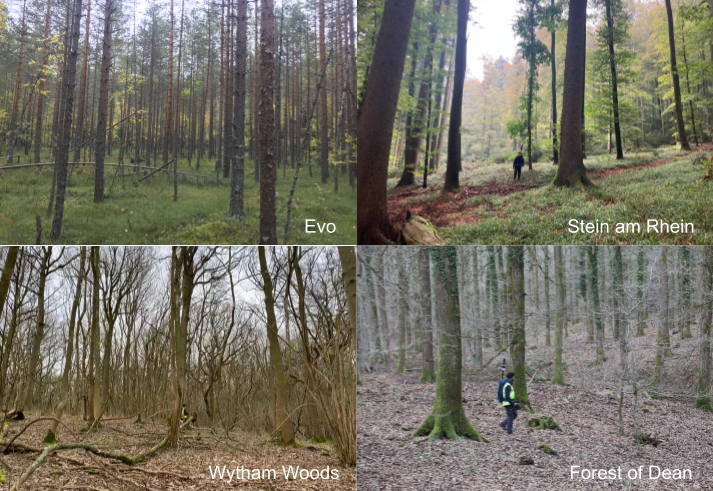
\includegraphics[width=\columnwidth]{pics/exp_0_missions_dataset.pdf}
  \caption{Illustrative examples of four forests used in the experiments. From top left to bottom right: Evo (Finland, May), Stein am Rhein (Switzerland, Sep), Wytham Woods (UK, Feb), and Forest of Dean (UK, March). The datasets were collected using backpack-LiDAR systems across different seasons and forest types.}
  \label{fig:missions_dataset}
\end{figure}


% First experiment: descriptors
\section{Place Recognition Descriptors}
\label{sec:exp_desc_analysis} 
In this experiment, we evaluated the descriptors of four different place recognition models (Logg3dNet, EgoNN, ScanContext, STD) focusing on their ability to accurately capture loop-candidates in forest environments. Logg3dNet and EgoNN models are learning-based methods and were pre-trained on the Wild-Places dataset. 
\subsection*{Datasets}
We collected the dataset with two different LiDAR sensors mounted on a backpack: Hesai XT32 and Hesai QT64  as discussed in previous \secref{sec:system_setup}. Note that Wild-Place\cite{knights2023icra} dataset was collected using a inclined VLP-16 LiDAR mounted on spinning motor. This enabled capturing the canopy of the forest, which is difficult for our backpack LiDAR setup. Below summarises the characteristic of different forests:
\begin{itemize}
  \item \textbf{Evo:} Evo dataset was collected in forests in Finland. The dataset was collected in May using the Hesai XT32 LiDAR sensor. The forest is characterized by tall coniferous trees with medium tree density.
  
  \item \textbf{Stein am Rhein:} Stein am Rhein dataset was collected in a forest in Switzerland in October. The dataset was collected using the Hesai XT32 LiDAR sensor. It displays mixed species and bushes with a low tree density.   

  \item \textbf{Wytham Woods:} Wytham Woods dataset was collected in a densely wooded area in the UK in February. The dataset was collected using the Hesai QT64 LiDAR sensor. It is characterized by a high tree density with complex terrains featuring hills and valleys.
  
  \item \textbf{Forest of Dean:} Forest of Dean dataset was collected in a forest in the UK in March. The dataset was collected using the Hesai QT64 LiDAR sensor. The dataset displays a sparser plantation with a low tree density. 

  \item \textbf{Wild-Place:} Wild-Place dataset was collected in a forest in Australia over different seasons. The dataset was collected using a VLP-16 LiDAR sensor mounted on a spinning motor. The trajectories were along the open access roads and the forest canopy was captured. The dataset is characterized by a low tree density.  
\end{itemize}

% \begin{table}[ht]
%   \centering
%   \label{tab:lidar_specs}
%   \begin{tabular}{|p{2.5cm}|p{2cm}|p{2.3cm}|p{2.3cm}|c|}
%     \hline
%     \centering \textbf{Location} & \centering  \textbf{LiDAR} & \centering  \textbf{Field of View (\textdegree)} &\centering  \textbf{Effective Range (m)} & \textbf{Tree Density} \\
%     \hline
%     \centering Wild-Place & \centering VLP-16 & \centering 30  & \centering 50 & Low \\
%     \hline
%     \centering Evo &  \centering XT32 &\centering 30 &\centering 50 & Medium \\
%     \hline
%     \centering Stein am Rhein &\centering  XT32 & \centering 30 & \centering 50 & Low \\
%     \hline
%     \centering Wytham Woods &\centering  QT64 &\centering 100 &\centering 30 & High \\
%     \hline
%     \centering Forest of Deans &\centering QT64 &\centering 100 &\centering 30 & Low \\
%     \hline
%   \end{tabular}
% \caption{Datasets and LiDAR specifications.}
% \end{table}


\begin{table}[htbp]
  \centering
  \caption{Evaluation results for a sequence of datasets.  Abbreviations used are as follows: Avg (Average), Online (Online SLAM), Offline (Offline multimission), Reloc. (Relocalization), Indiv. (Individual), Indiv.pc (Individual point clouds) }
  \label{tab:eval_sequence}
  \small
  \centering
  \begin{tabular}{>{\centering\arraybackslash}m{1.5cm} >{\centering\arraybackslash}m{1.5cm} >{\centering\arraybackslash}m{1.5cm} >{\centering\arraybackslash}m{1.5cm} >{\centering\arraybackslash}m{1.5cm} >{\centering\arraybackslash}m{1.5cm} >{\centering\arraybackslash}m{1.5cm}}
  \toprule
  Dataset  & Eval Modes & Avg. Mapping area(ha) & Avg. Duration (min) & Avg. \#Indiv. pc  & Avg.\#points per indiv.pc  \\
  \midrule
  Evo  & Desc. Online. Offline. & 0.74 ha   & 24 min & 969 &  110k \\
  \midrule
  Stein am Rhein  & Desc. & 0.27 ha & 13 min & 363 &  120k \\
  \midrule
  Wytham Woods & Desc. Online. Offline.  & 1.2 ha & 22 min& 707 & 55k \\
  \midrule
  Forest of Deans & Online. Offline. Reloc. & 0.45 ha  & 17 min & 649 & 50k \\
  \midrule
  Wild-Place & Desc. & Perimeter 3.17km  & 48 min & 5805 & 300k \\
  \bottomrule
  \end{tabular}
\end{table}

\subsection*{Precision-Recall Curves}
Precision-recall curves (See \figref{fig:pr_curves}) show how accurately (precision) and frequently (recall) each  model detects correct loop candidates within a reasonable distance threshold (here set to 10\,m) at various descriptor thresholds $\tau_{s}$ in four different forests. Among positive candidates   (whose descriptor distance < $\tau_{s}$ ), we classify them into true positive(\emph{TP}) and false positive(\emph{FP}) depending on whether the candidate is actually located within the loop-closure distance threshold, 10 meter. 
Similarly, among negative candidates, we classify them into true negative(\emph{TN}) and false negative(\emph{FN}) depending on their true location. Thus:
\[ Precision = \frac{TP}{TP + FP} \quad   \ Recall = \frac{TP}{TP + FN} \]

From the precision-recall curves (\figref{fig:pr_curves}), it is evident that Logg3dNet consistently outperforms the other models across the four different forests. Particularly, on the Evo and Stein am Rhein datasets, where a longer range with narrow field of view Hesai XT32 LiDAR was employed, Logg3dNet showed the best performance both in terms of precision and recall, without experiencing any sudden drops in precision.
In contrast, ScanContext demonstrates a significant decrease in precision, attributed to a limited vertical field of view of LiDAR sensor. In more challenging scenarios such as Wytham Woods characterized by complex terrains featuring hills and valleys with dense tree clutter captured with a wide field of view QT64 LiDAR, handcrafted models show a notable decline in performance. However, Logg3dNet remains robust, successfully retrieving a substantial portion of correct loop-candidates, achieving a 70\% precision at a 50\% recall rate. 
\begin{figure}[htbp]
  \centering
  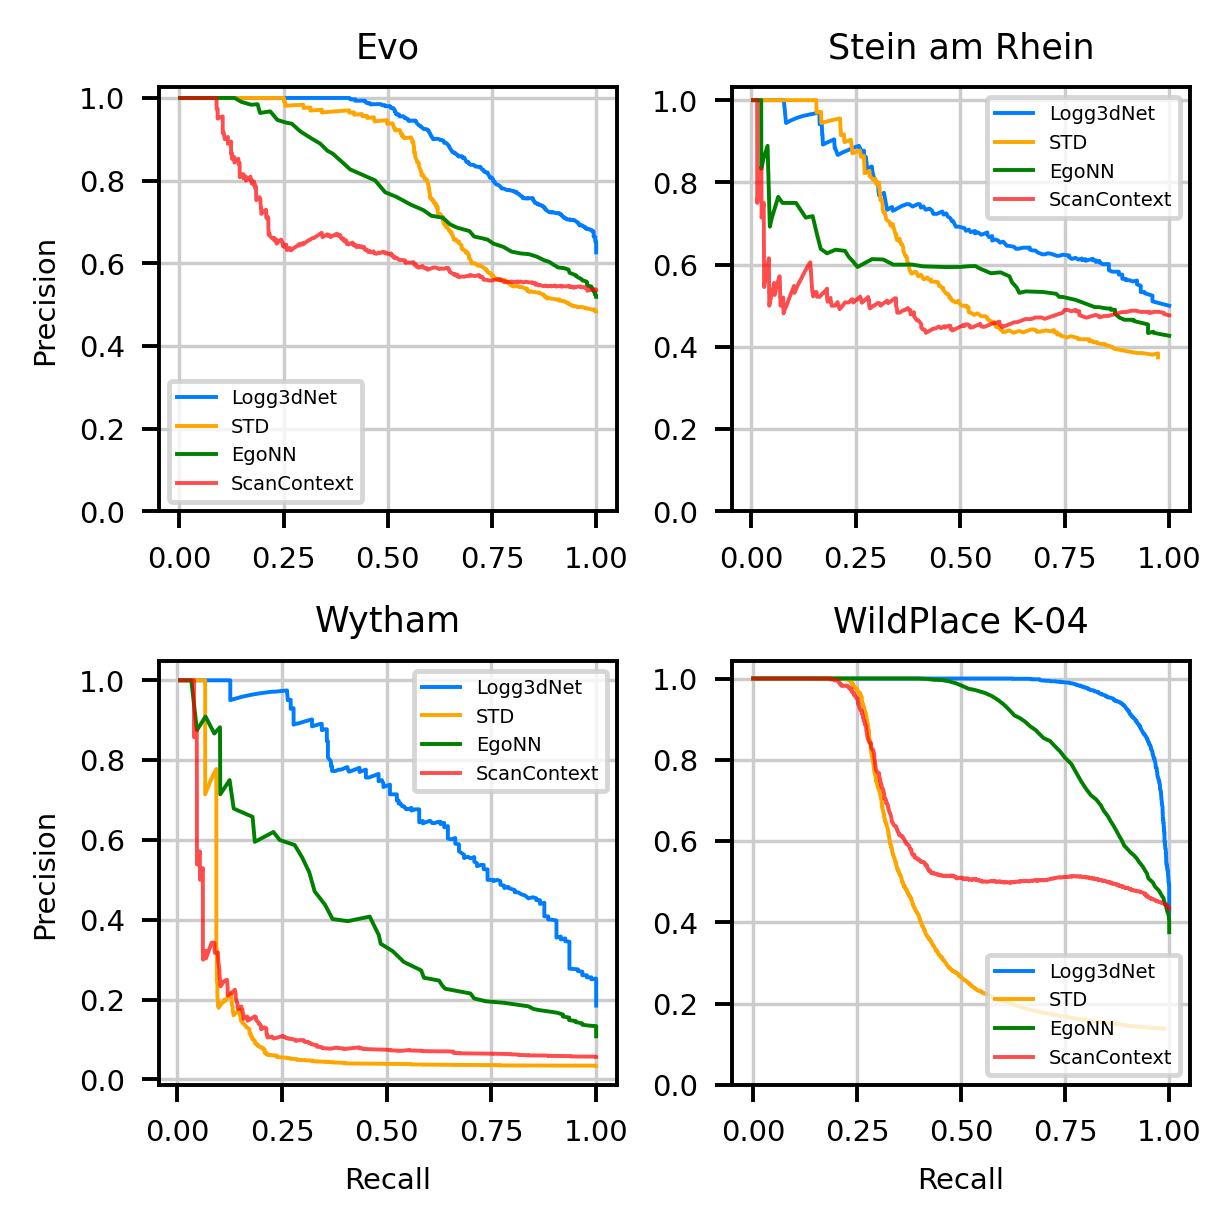
\includegraphics[width=0.9\linewidth]{pics/exp_1.1_pr_curves}
  \caption{Precision-recall curves on four different forest datasets. Evo (Finland, May), Stein am Rhein (Switzerland, Oct), Wytham woods (UK, Feb), Wild-Places \cite{knights2023icra} (Australia).
  Evo and Stein am Rhein datasets were collected by Hesai XT32, and Wytham woods dataset was collected by Hesai QT64. Datasets were collected by backpack-LiDAR within dense forests. Only top-1 candidate within 10\,m of the ground truth position is regarded as a true positive candidate.}
  \label{fig:pr_curves}
\end{figure}
% \mfallon{I get to this bit and there is just a hole in the work because nothing about Logg3dNet's algorithm is ever discussed. There is no tuning or ablation. It just presented `as is'.}
\subsection*{Heatmaps}
To further analyze the distinctiveness of each descriptor, we measured the descriptor distances between all query and database descriptors. This is shown in \figref{fig:heatmap_evo12} as a heatmap, which provides a visual representation of the discriminative potential of each descriptor. Consistent with the precision-recall curves, Logg3dNet descriptors exhibited higher similarity with the ground truth heatmap as observed in the highlighted areas, indicating a high true-positive rate and low false-positive rate, respectively. This implies that Logg3dNet descriptors can effectively detect corresponding loop-candidates during revisits, whereas EgoNN and ScanContext tend to be less discriminative, often returning numerous false-positive candidates. Based on this evidence, we chose Logg3dNet as main the place recognition method for the rest of the experiments.
\begin{figure}[htbp]
  \centering
  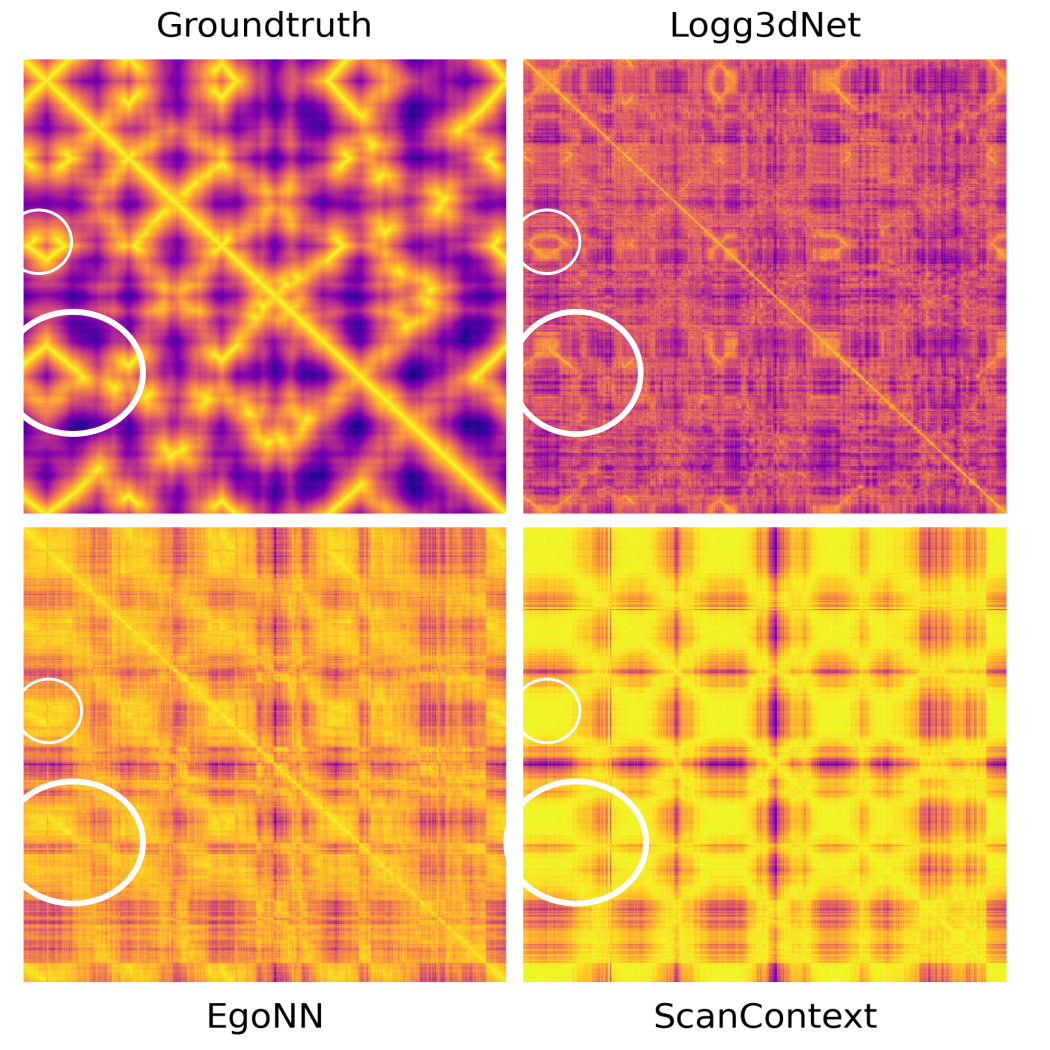
\includegraphics[width=0.9\linewidth]{pics/exp_1.2_heatmap_evo12_plasma_edit}
  \caption{Heatmaps depicting descriptor distances for the Evo dataset. Yellow hues denote a high descriptor similarity between scans, whereas purple indicates the low similarity. Patterns more closely resembling the ground-truth (top-left) indicate better descriptor performance. Logg3dNet descriptors shows the most similar patterns, whereas ScanContext descriptors are least discriminative among these models. We use $\tau_{s}$ that corresponds to the $F_1$-max score in evaluation.}
  \label{fig:heatmap_evo12}
\end{figure}





%%% Second experiment: Online SLAM
\section{Online Single Mission SLAM}
\label{sec:exp_online_slam}
In this experiment, we investigate the online place recognition capability of our system, wherein loop closures from the place recognition module are integrated into the SLAM system. The database $D$, is incrementally built as the sensor moves through the environment. When matching, we exclude the most recent 30 seconds of data to prevent loop closures with immediately recent measurements.
\begin{figure}[htbp]
  \centering
  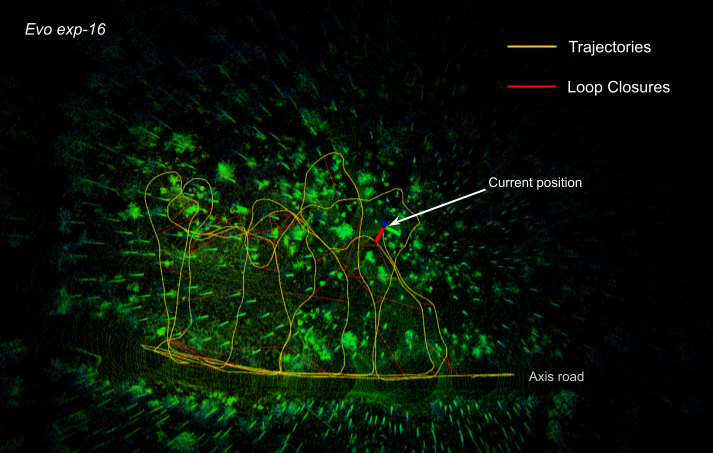
\includegraphics[width=0.9\columnwidth]{pics/exp_2_0_rviz.png}
  \caption{Online SLAM Operation visualizations through Rviz on Evo exp16 sequence. }
  \label{fig:exp_2_0_rviz}
\end{figure}



\subsection*{Online Place Recognition}
% Interpret results exp_2_1
\figref{fig:exp_2_1_evo_online} presents an illustrative example of online SLAM performance on the Evo datasets, depicting the sets of loop candidates after each verification step. Initially, many loop closure candidates are proposed (shown in blue) under a descriptor matching threshold $\tau_{s}$ of $F_1$-max score. Loop closures beyond a conservative estimate of \SI{20}{\meter} are rejected using the odometry information. After this, a subset of loop closure candidates are identified using RANSAC matching (highlighted in orange), and finally, a refined set of loop closures that pass the consistency and ICP steps are integrated into the SLAM framework. Final loop closures (shown in red) are one of ICP verified loop candidates by checking pose graph density to avoid over-constraining the pose graph. We tested on two sequences on Evo and Wytham dataset. 
\newline
\textbf{Evo}\hspace{0.5em} We tested on Evo dataset as shown \figref{fig:exp_2_1_evo_online}. Evo16 sequence is densly scanned where each zigzag turn is about 10-15m apart, whereas Evo12 is mapped sparsely with about 20-30m apart. For Evo16, we can observe frequent loop candidates upto \SI{20}{\meter} between each zigzag turn, whereas for Evo12, loop closures are less frequent and more candidates (above \SI{15}{\meter}) are strongly rejected before RANSAC registration(Blue lines). In summary, we observed that the system can reliably detect loop closures inside the dense forest in both cases and correct the drift. 
\begin{figure}[htbp]
  \centering
  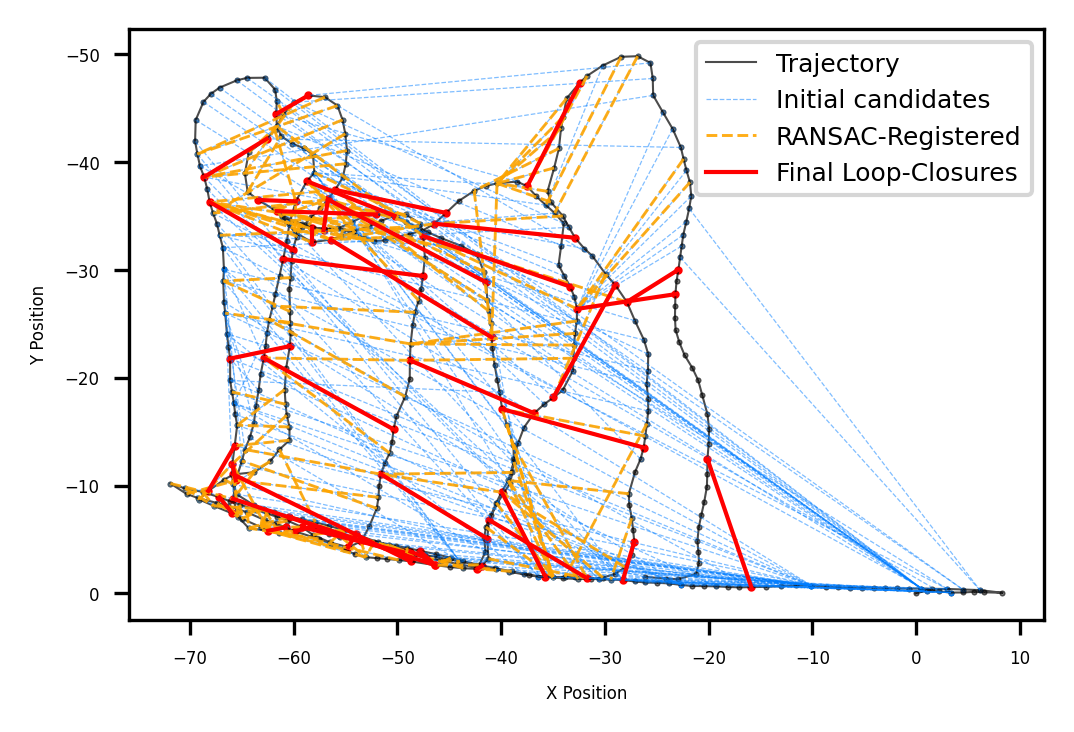
\includegraphics[width=0.53\columnwidth]{pics/exp_2_1_evo16_online2.png}
  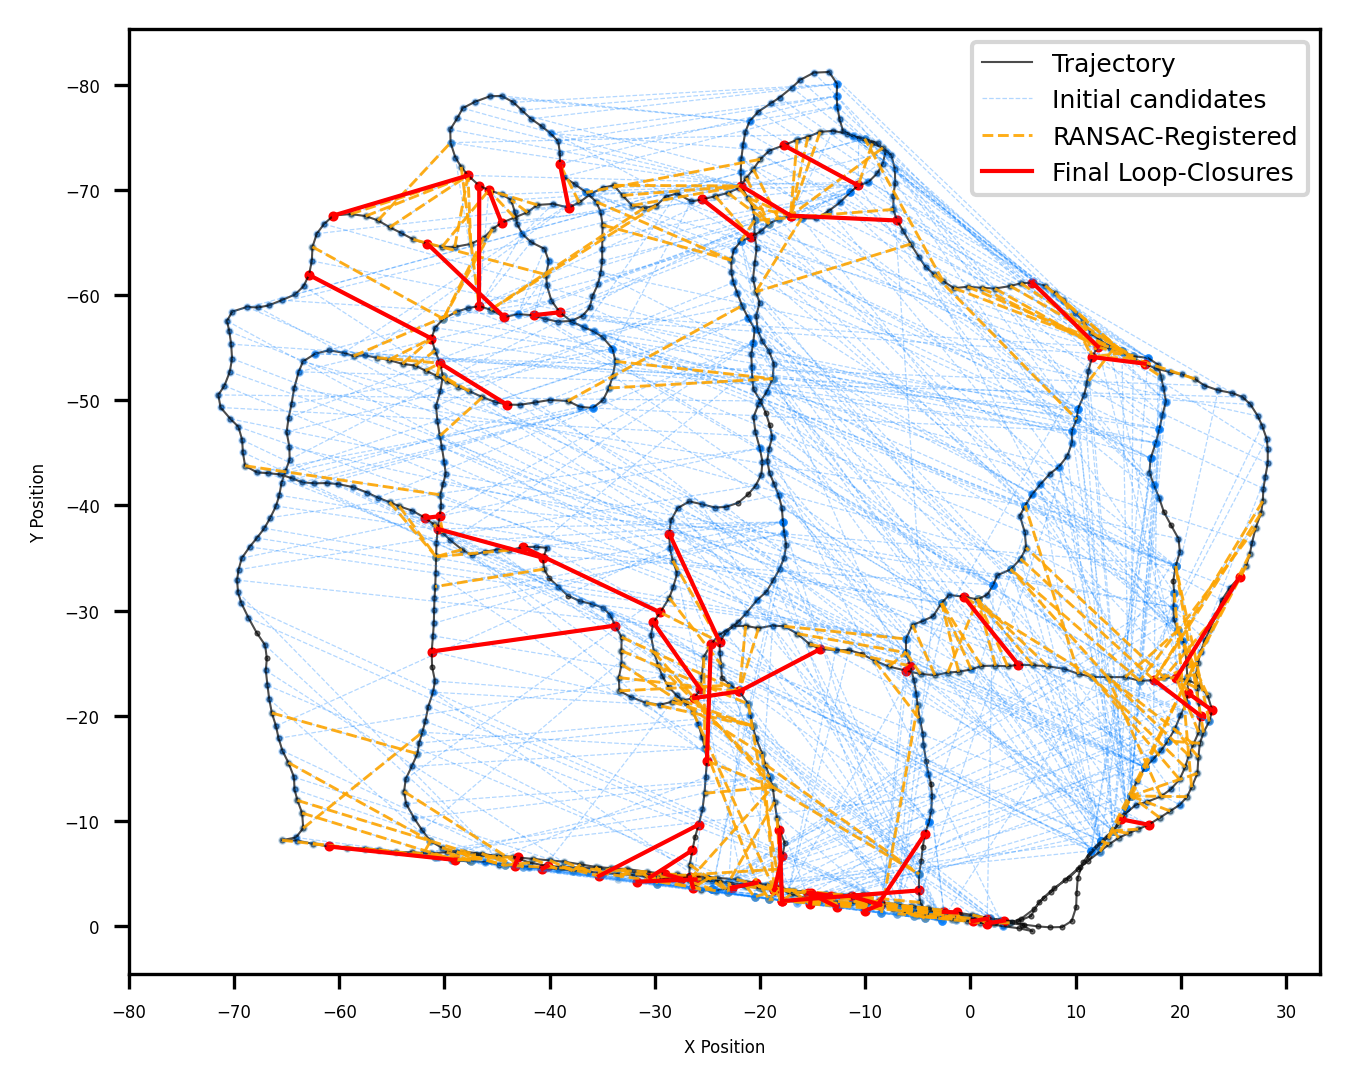
\includegraphics[width=0.46\columnwidth]{pics/exp_2_1_evo12_online.png}
  \caption{Online SLAM results on Evo dataset. Evo16(Left) and Evo12(Right). Initial candidates (Blue) proposed by descriptor distance and odometry check. Yellow lines are successfully RANSAC-registered candidates which passed SGV and pairwise consistency checks. Red lines are final loop closures after ICP verification and checking constraints density in pose graph.}
  \label{fig:exp_2_1_evo_online}
\end{figure}
\newline
\textbf{Wytham Woods}\hspace{0.5em} We further tested on more challenging dataset, Wytham Woods, which is a densely wooded area with uneven terrain, including hills. In \figref{fig:exp_2_1_ewytham_online}, we observed that there are still enough numbers of correct RANSAC-registered loop candidates, but ICP could not fine-register them. For example, regarding Mission D(top figure) of \figref{fig:exp_2_1_ewytham_online}, our system correctly detected loop candidates and RANSAC registered them (Yellow lines) at each turns. However, the ICP rejected almost all candidates due to very small number of overlapping point clouds between two scans (usually 2k-3k out of 20k points, $\sim$\SI{10}{\percent} overlaps). Unfortunately, lowering ICP thresholds to less than $\sim$ 3k points resulted in failure of system. Our system suffers from high outliers rate due to occlusions and sparse point clouds at the far distance making ICP registration challenging. As a result, our system partly corrected the drifts in both sequences, failing to correct drifts at the start. 
\begin{figure}[htbp]
  \centering
  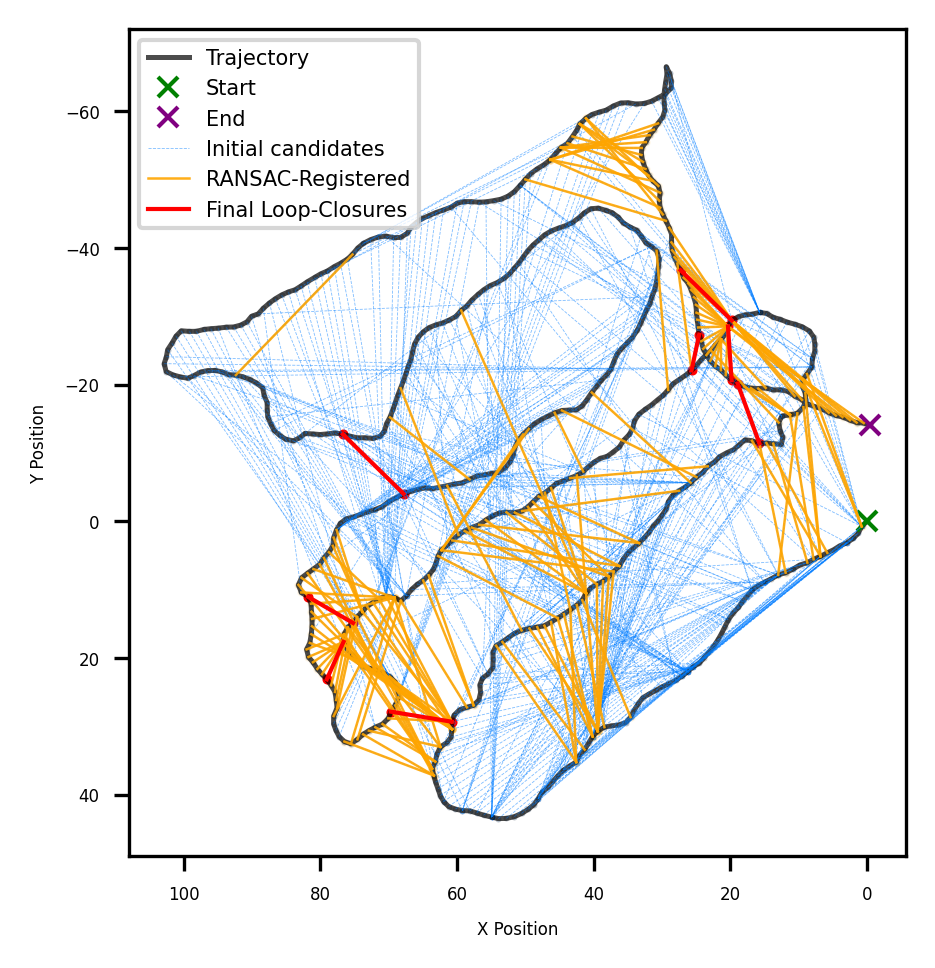
\includegraphics[width=0.49\columnwidth]{pics/exp_2_1_wytham_D.png}
  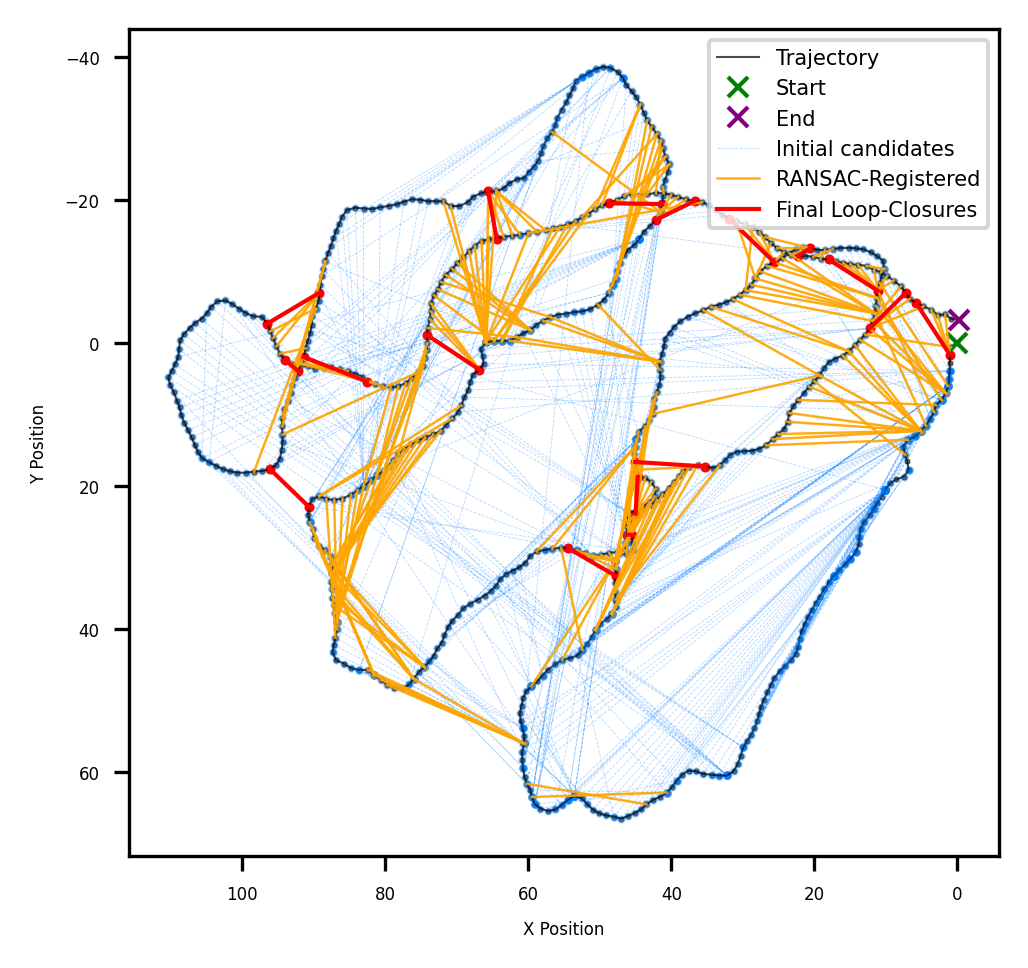
\includegraphics[width=0.49\columnwidth]{pics/exp_2_1_wytham_C.png}
  \caption{Online SLAM results on Wytham Woods, two sequences Mission D(Left) and Mission C(Right) are shown. Blue lines are initial candidates proposed by descriptor distance and odometry check. Yellow lines are successfully RANSAC-registered candidates which passed SGV and pairwise consistency checks. Red lines are final loop closures after ICP verification and checking constraints density in pose graph.}
  \label{fig:exp_2_1_ewytham_online}
\end{figure}


\subsection*{Loop Closure Statistics}
% Present results in exp2_2
Alongside visual illustrations of loop closures, we conducted a comprehensive analysis of loop closure statistics based on distance and viewpoint angles, shown \figref{fig:exp_2_2_loop_closure_histograms}. Our findings show that the system can successfully identify loop closure pairs across considerable baseline distances (\SIrange{10}{20}{\meter}). 
\newline
\textbf{Baseline distance}\hspace{0.5em} We observed that despite the large baseline, a significant portion of initial candidates can be registered using RANSAC-based matching, indicating that the correspondences are accurate. However, the proportion of candidates verified by ICP decreases as the distance between scans increases. Specifically, when scans are \SI{10}{\meter} apart, $\sim$\SI{60}{\percent} of RANSAC-registered candidates are successfully verified by ICP, and when \SI{15}{\meter} apart, only $\sim$\SI{40}{\percent} remains verified. This decrease is due to the diminishing overlap ratio between corresponding scans with increasing distance, making convergence of ICP challenging. \\
\textbf{Viewpoints difference}\hspace{0.5em} Similarly, in terms of viewpoint orientation difference, we observed that a large proportion of the loop candidates up to \SI{90}{\degree} difference are verified both at the RANSAC-registration and ICP-based checks. However, we observed a degradation of performance over \SI{90}{\degree}, which can be attributed to the occlusions in the scans present at large orientation differences. Nonetheless, despite this degradation, the number of final loop closures integrated into the SLAM system proved to be sufficient for correcting the drift.   

\begin{figure}[htbp]
  \centering
  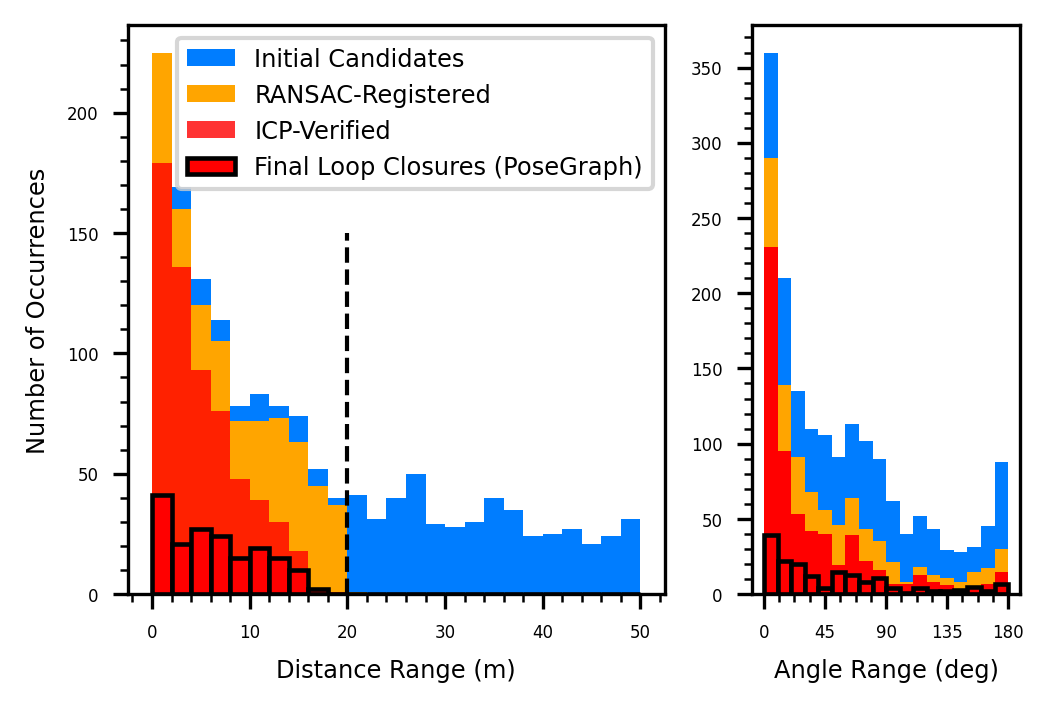
\includegraphics[width=0.85\columnwidth]{pics/exp_2_2_loop_closure_histograms}
  \caption{Loop closures distribution by distance and angle at various stages of the pipeline on Evo dataset.
   Initial candidates based on descriptor distance are shown in blue. Candidates beyond \SI{20}{\meter} are rejected using odometry information. Candidates within \SI{20}{\meter} undergo RANSAC pre-registration with additional verification steps of SGV\cite{vidanapathirana2023ral} and pairwise checks (Yellow). Then these candidates are refined using ICP fine-registration (Red), and final loop closures in the pose graph after checking constraints density in pose graph (red with black outlined).}
  \label{fig:exp_2_2_loop_closure_histograms}
\end{figure}



\subsection*{Model Comparison}
\textbf{ScanContext}\hspace{0.5em} So far we have shown capability of Logg3dNet reliably finding loop closures inside the forest. We now shows ScanContext implemented on our SLAM system on Evo16 dataset to compare with Logg3dNet. It was evident ScanContext shows a drop in performance in \ref{sec:exp_desc_analysis}, and now we evaluate if ScanContext can detect any loop candidates and find 6DoF transformation reliably inside the forest.  
\begin{figure}[htbp]
  \centering
  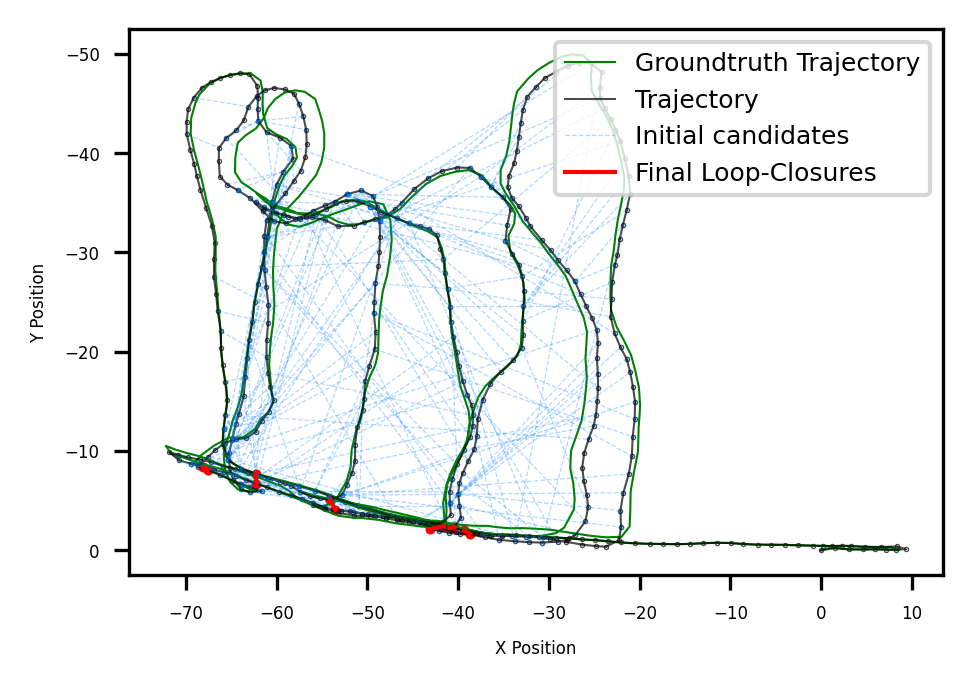
\includegraphics[width=0.75\columnwidth]{pics/exp_2_sc_loop_closure.png}
  % 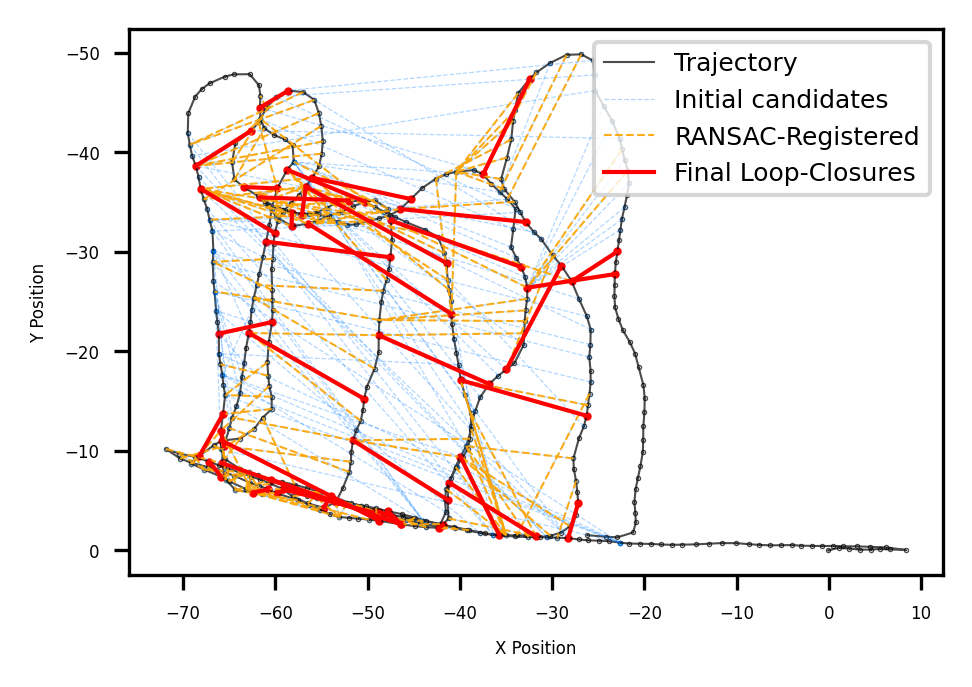
\includegraphics[width=0.49\columnwidth]{pics/exp_2_logg3dnet_loop_closure.png}
  \caption{Loop closures with ScanContext on Evo exp16 dataset. ScanContext could not detect any loop closures inside the dense forest but only in open access roads, whereas Logg3dNet successfully found loop closures inside the forest. Also ScanContext only detected loop closures within 3m(same location), whereas Logg3dNet detected loop closures upto 15m. Finally, Scancontext accumulated drift over time.}
  \label{fig:exp_2_3_loop_closure_comparison}
\end{figure}

From \figref{fig:exp_2_3_loop_closure_comparison}, we can observe that ScanContext could not detect any loop closures inside the dense forest producing very high number of false positives (shown in blue lines), and could detect only in open access roads. Among those loop closures along open access roads, ScanContext detected only within 3m(same location). Finally, Scancontext accumulated drift over time while Logg3dNet corrected drifts. This shows very limited capability of ScanContext compared to Logg3dnet, and this experiment validates the robustness of Logg3dNet compared to ScanContext (handcrafted method) in dense forest environments.



% Third experiment: Offline Multi-Mission SLAM
%%% 
\section{Offline Multi-Mission SLAM} 
\label{sec:offline_multi_mission}
In this experiment, we showcased the ability of our approach to obtain loop closures between different mapping missions and to merge those missions into a common map. In this task, we employed tighter descriptor thresholds ($\tau_{s}$) compared to the online SLAM task, in order to reduce the number of false positive loop candidates.
Below shows the results of merging different sequences within three different datasets: Wytham Woods, Evo, and the Forest of Dean. Each individual mission covers approximately one hectare, with merged map areas ranging from three to five hectares.
\newline
\textbf{Evo, \figref{fig:exp_multi_mission_evo}}\hspace{0.5em} We tested the robustness of our system on the Evo multi-mission dataset, where the XT32 LiDAR was placed at a \SI{45}{\degree} inclination aimed at capturing the forest canopy. Despite the asymmetry in point clouds introduced by this inclination change, which primarily captured points in the forward direction, our approach successfully identified loop closures and achieved multi-mission map merging.
\begin{figure}[htbp]
  \centering
  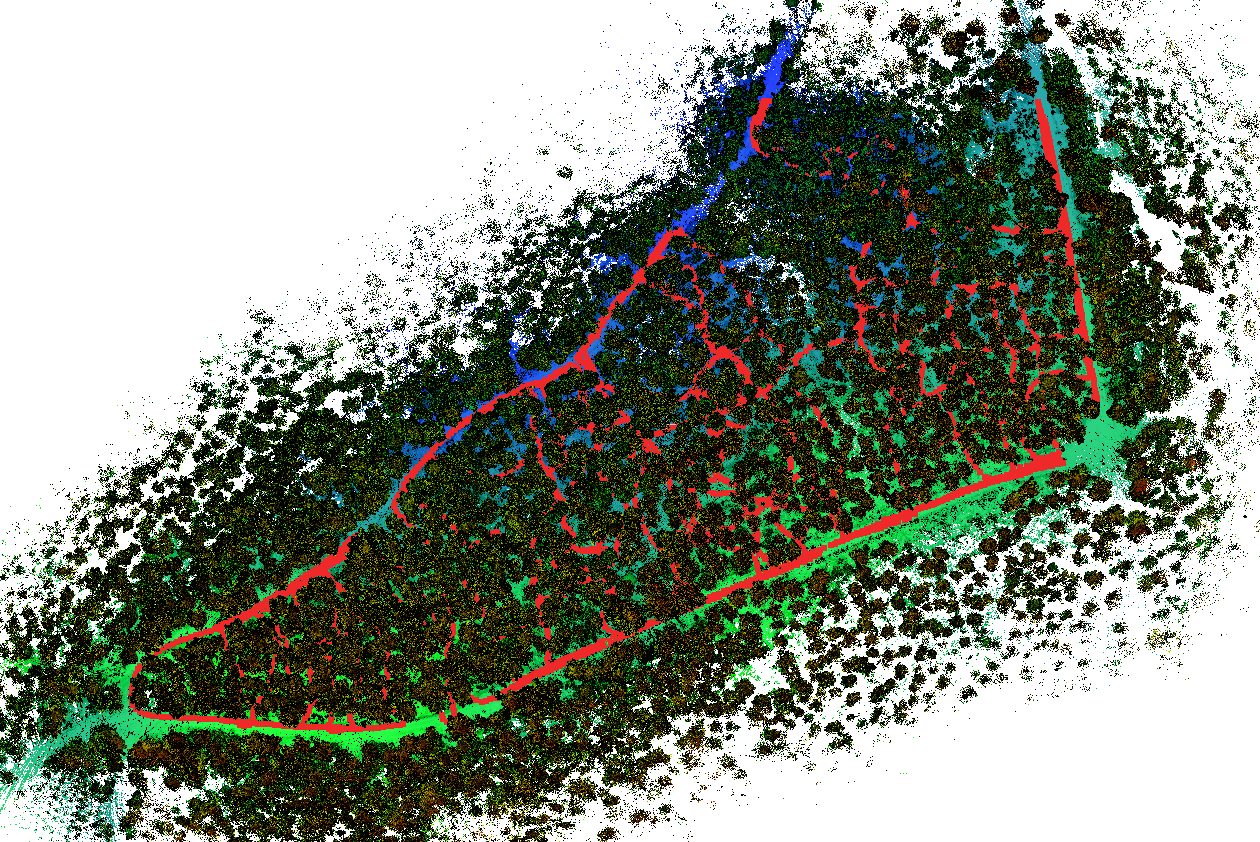
\includegraphics[width=\columnwidth]{pics/exp_3_offline_evo_pcd.png}
  % \caption{Offline multi-mission SLAM point clouds output.}
  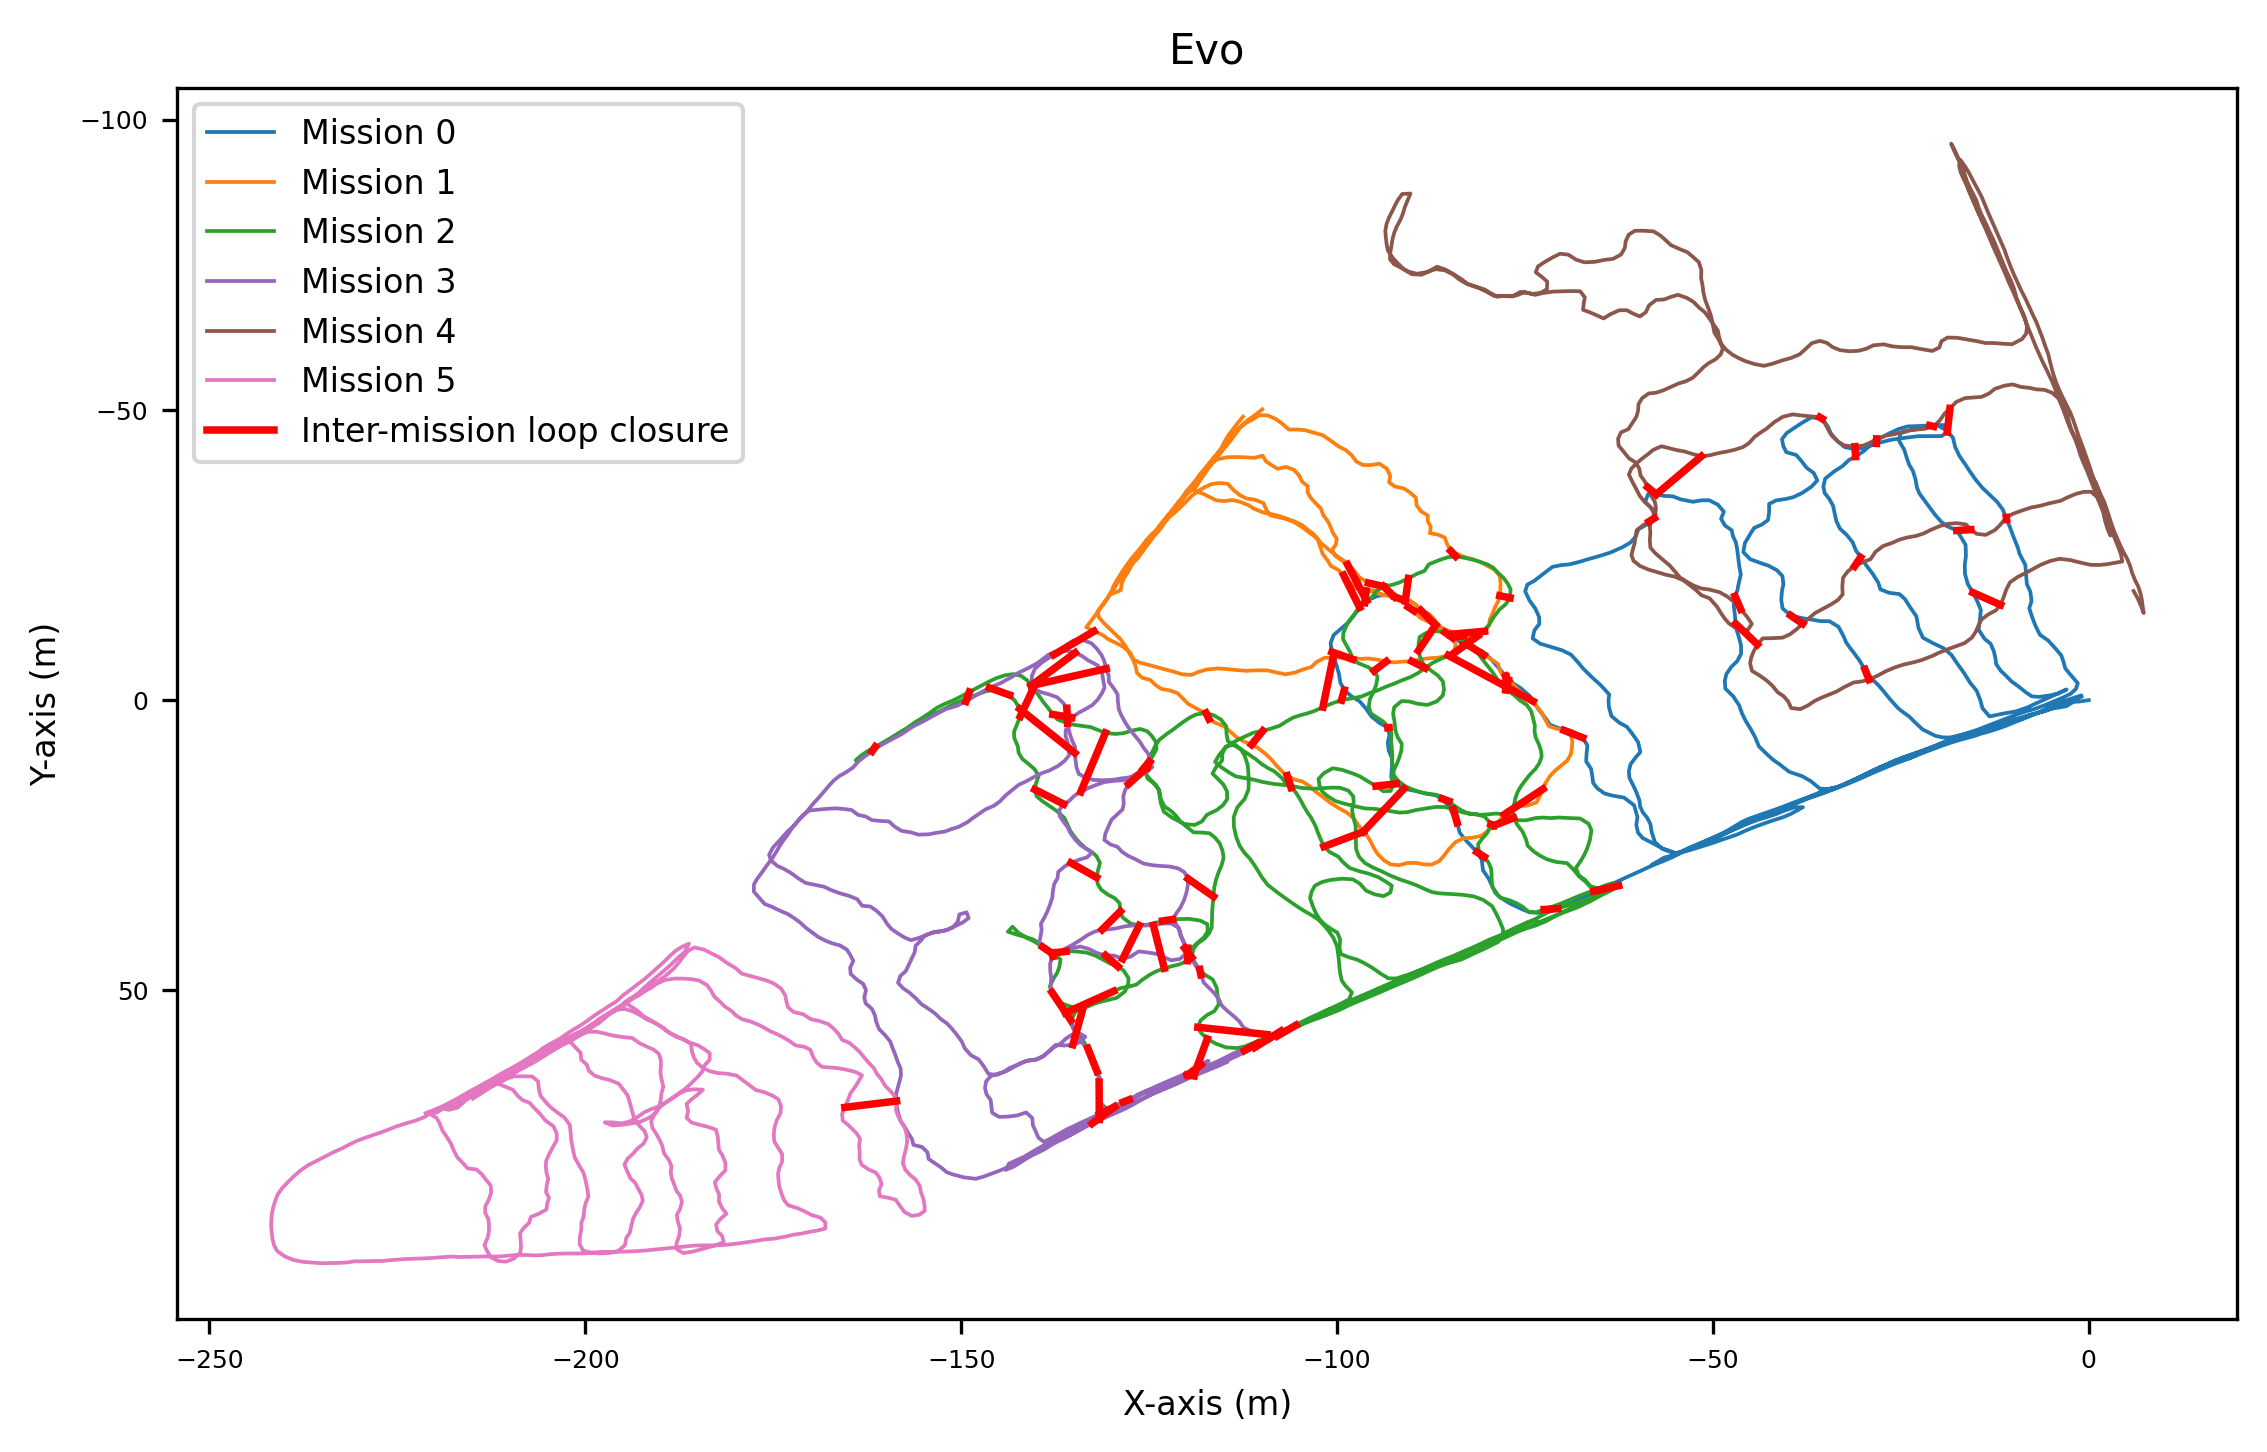
\includegraphics[width=\columnwidth]{pics/exp_3_1_multimission_slam_evo.png}
  \caption{Offline multi-mission SLAM (Evo).}
  \label{fig:exp_multi_mission_evo}
\end{figure}
\newline
\textbf{Wytham Woods, \figref{fig:exp_multi_mission_wytham}} \hspace{0.5em}  Wytham Woods were challenging due to the high tree density, foliage, and vegetation present captured with wide field of view Hesai QT64 LiDAR. Despite these challenges, our system successfully identified loop closures between different missions and merged them as shown in \figref{fig:exp_multi_mission_wytham}. During individual mission processing, slight drifts were noted at the beginning and end of each mission. However, through the multi-mission map merging process, the system successfully corrected these drifts occurring in overlapping areas. Nevertheless, minor drifts still persisted at the edges of the map. 
\begin{figure}[htbp]
  \centering
  \includegraphics[width=\columnwidth]{pics/exp_3_offline_wytham_pcd1.png}
  % \caption{Wytam Woods: Offline multi-mission SLAM pointclouds}
  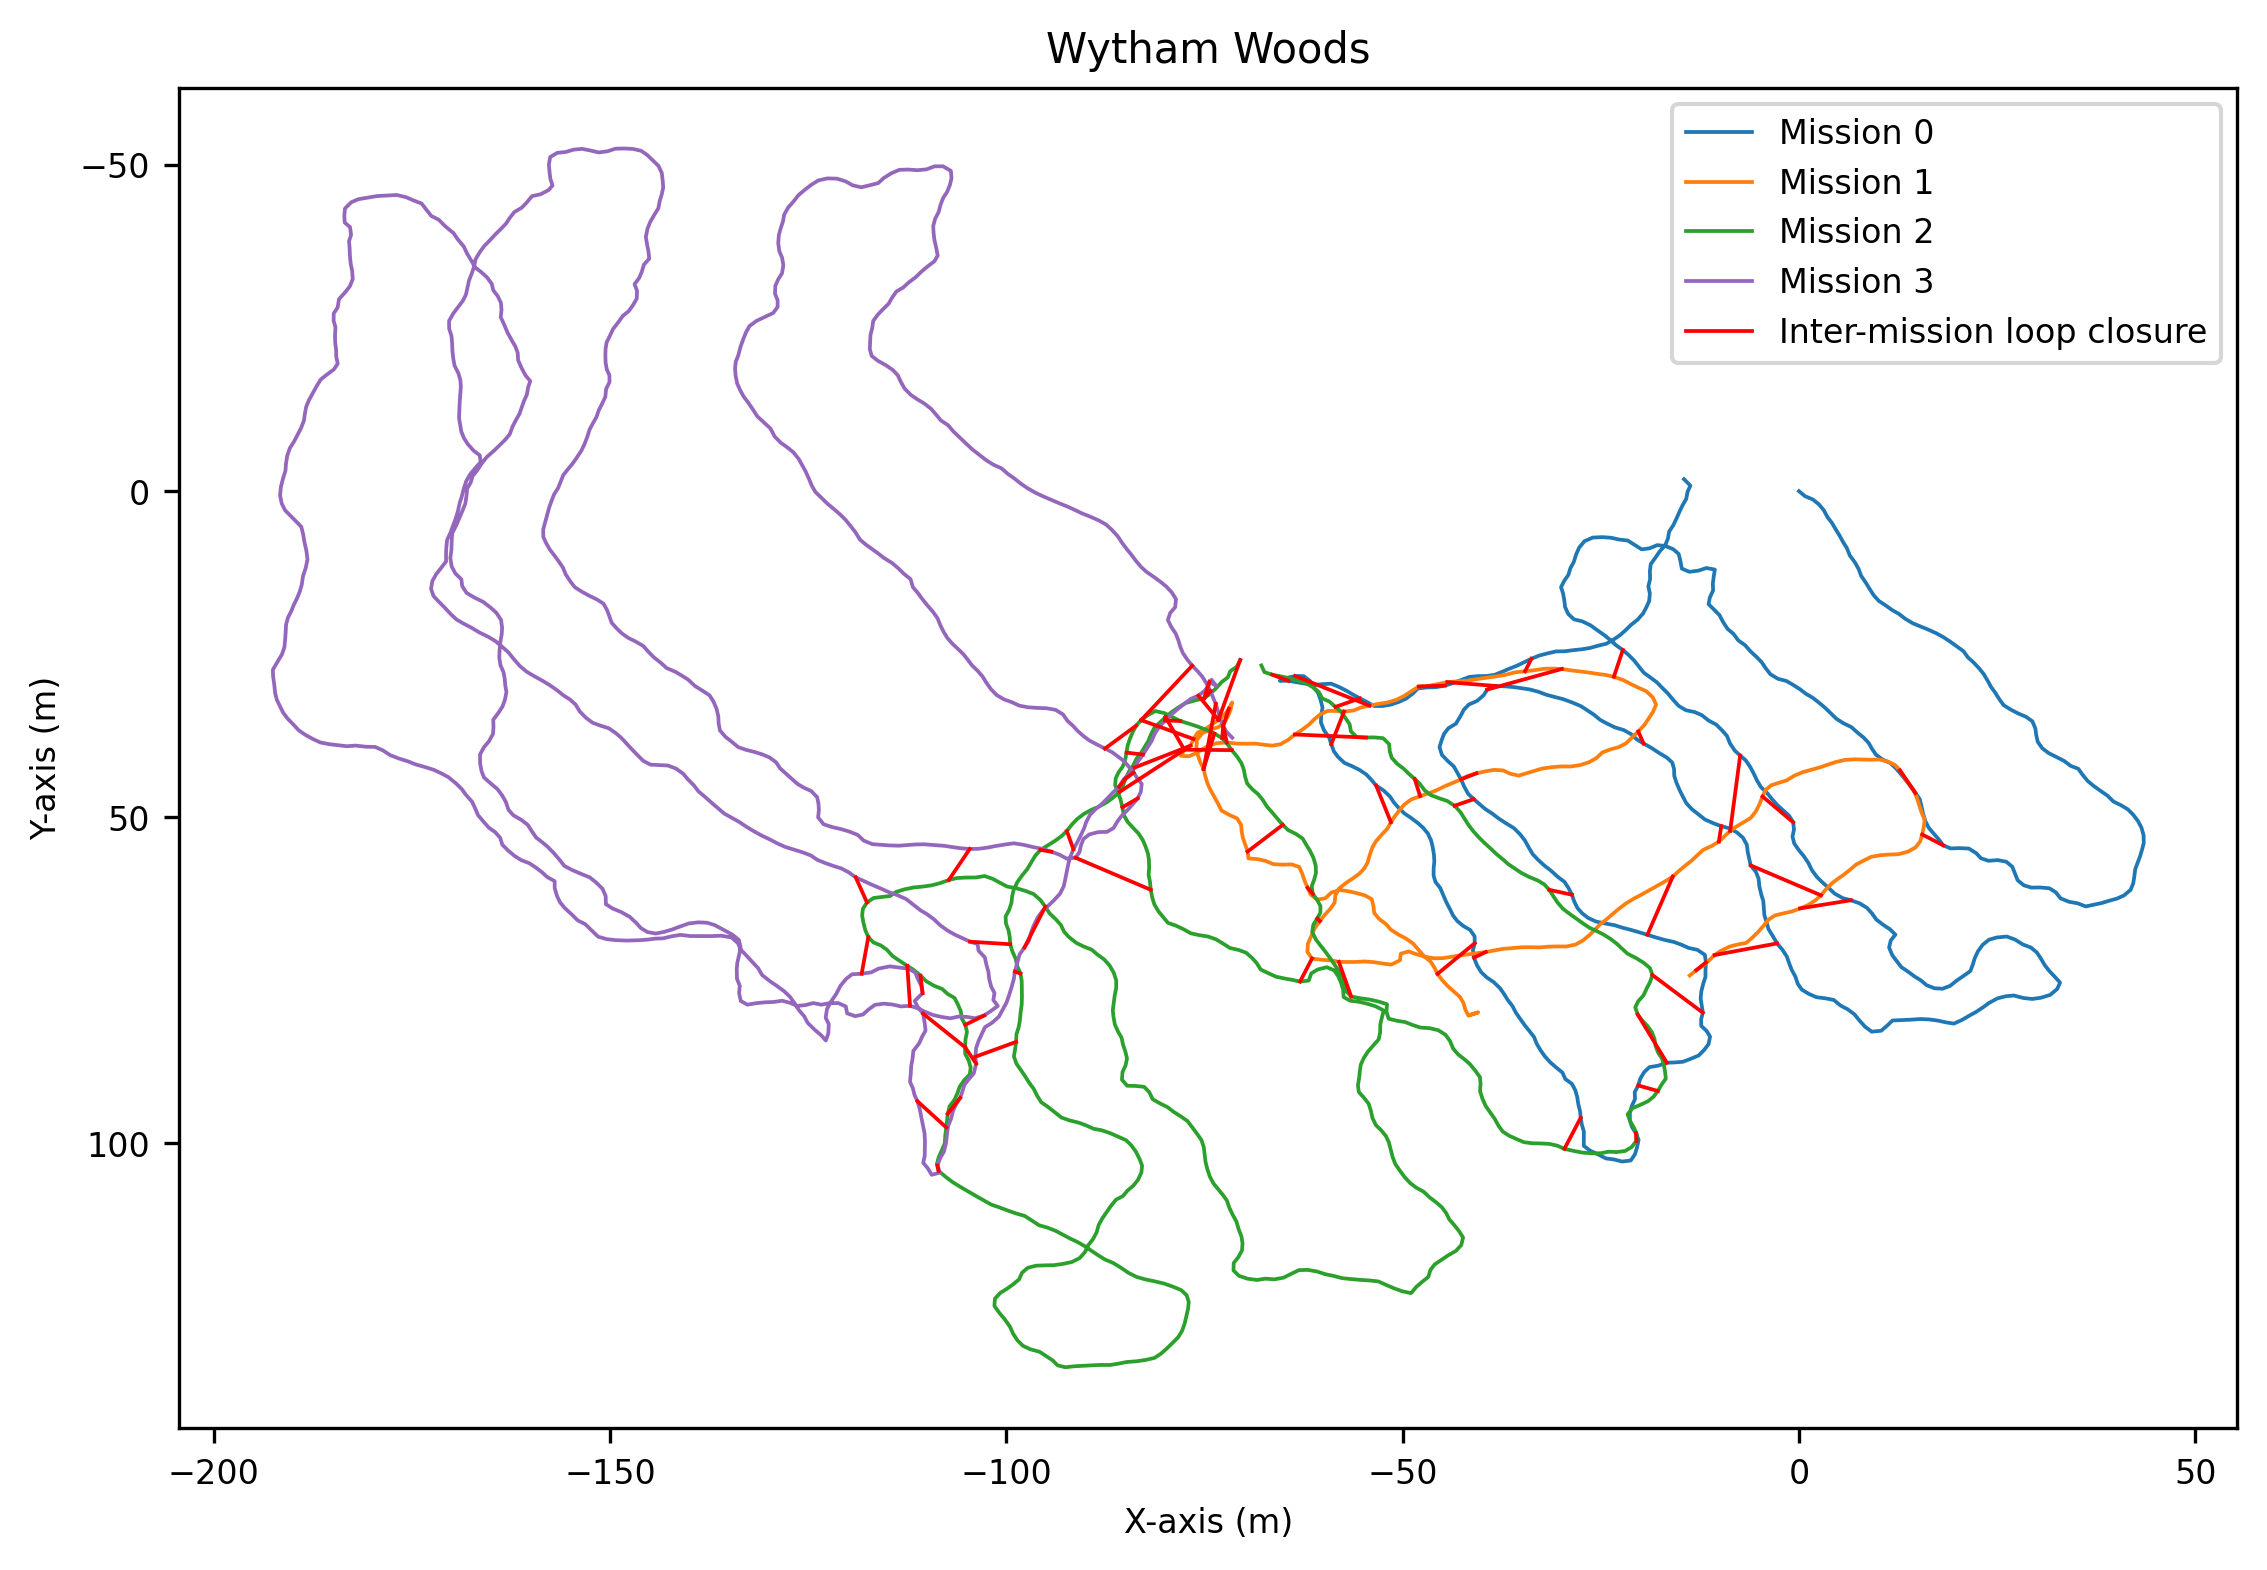
\includegraphics[width=\columnwidth]{pics/exp_3_1_multimission_slam_wytham.png}
  \caption{Wytham Woods: Offline multi-mission SLAM Loop Closures.}
  \label{fig:exp_multi_mission_wytham}
\end{figure}
\newline
\textbf{Forest of Dean, \figref{fig:exp_multi_mission_dean}}\hspace{0.5em} Forest of Dean is less dense forest and 3 missions were merged easily. We observed that there were more frequent \emph{intermission} loop closures in the Forest of Dean compared to Wytham in overlapping areas. 
\begin{figure}[htbp]
  \centering
  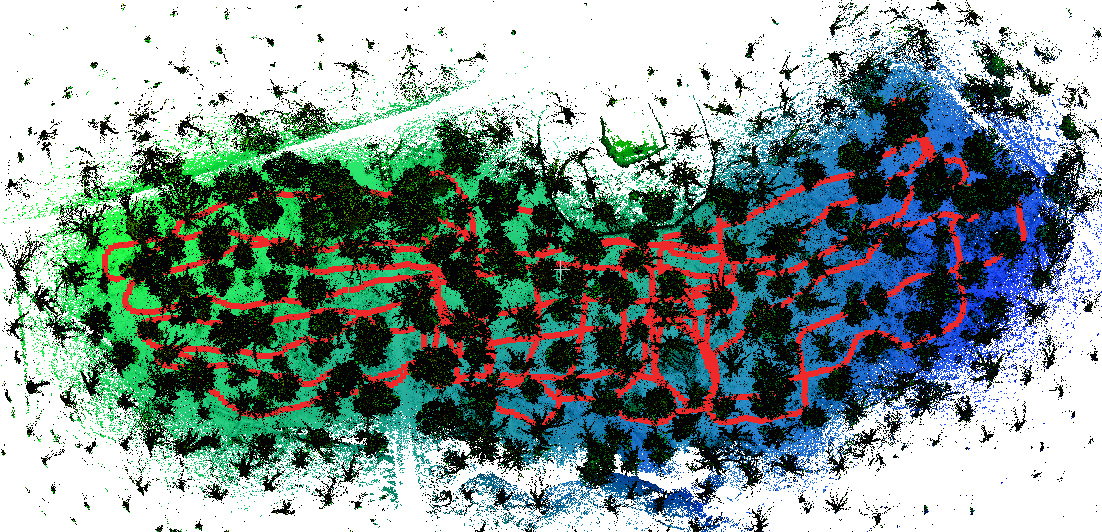
\includegraphics[width=\columnwidth]{pics/exp_3_offline_Dean_pcd3.png}
  % \caption{Forest of Dean: Offline multi-mission SLAM pointclouds}
  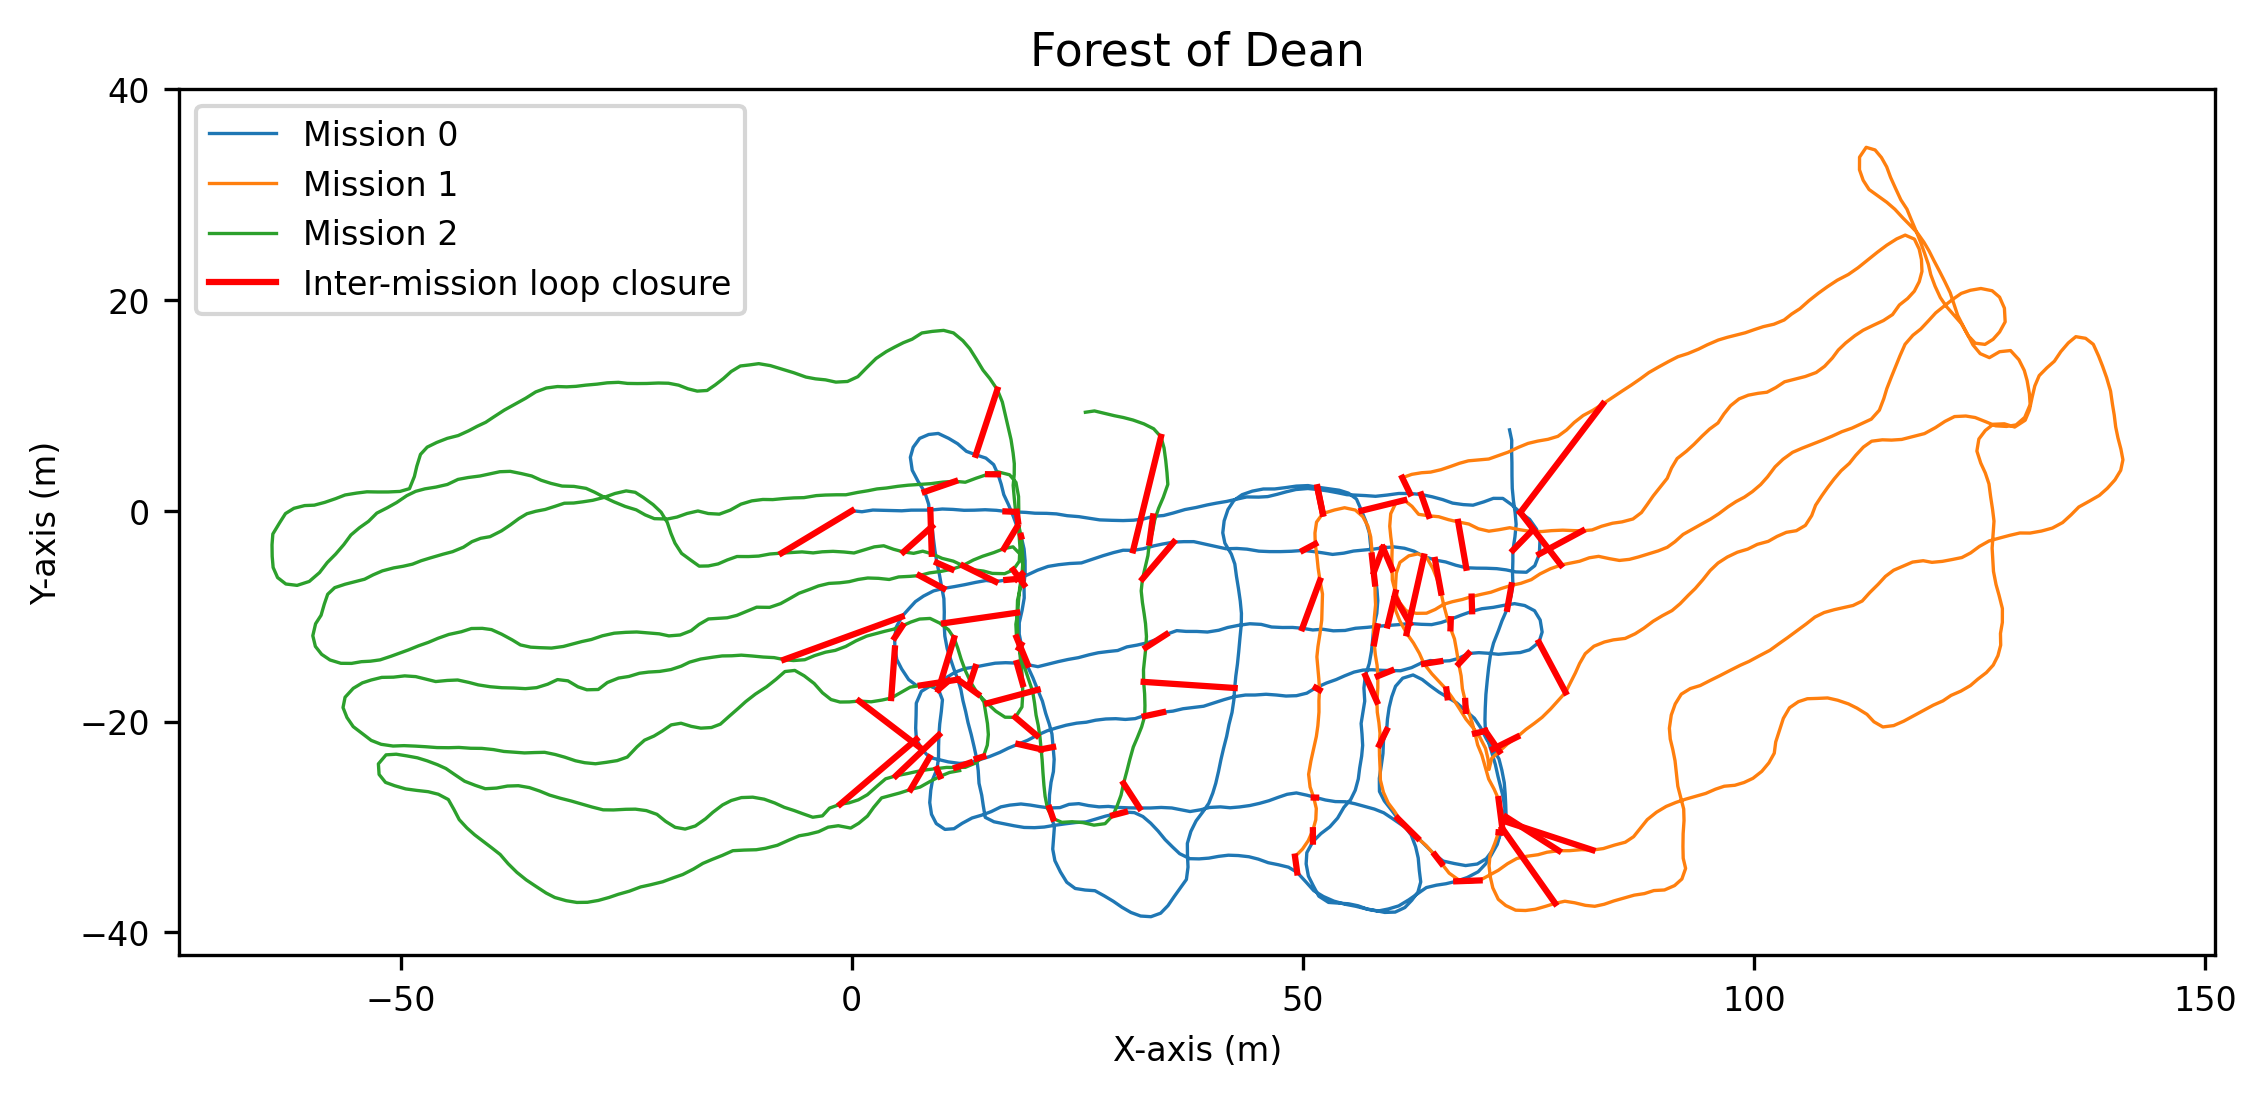
\includegraphics[width=\columnwidth]{pics/exp_3_1_multimission_slam_dean.png}
  \caption{Forest of Dean: Offline multi-mission SLAM Loop Closures.}
  \label{fig:exp_multi_mission_dean}
\end{figure}
\newline
\newline
\textbf{Map quality}\hspace{0.5em} We further analyzed the quality of the merged map by examining the point clouds of the merged map. We observed that the trunks of trees were very distinct, showing no evidence of drift. Circular shapes for tree trunks were clearly seen in the point clouds, indicating that the map scanned in different viewpoints were registered correctly. This is shown in \figref{fig:truk of trees} and \figref{fig:trunk of trees BV}.
\begin{figure}[htbp]
  \centering
  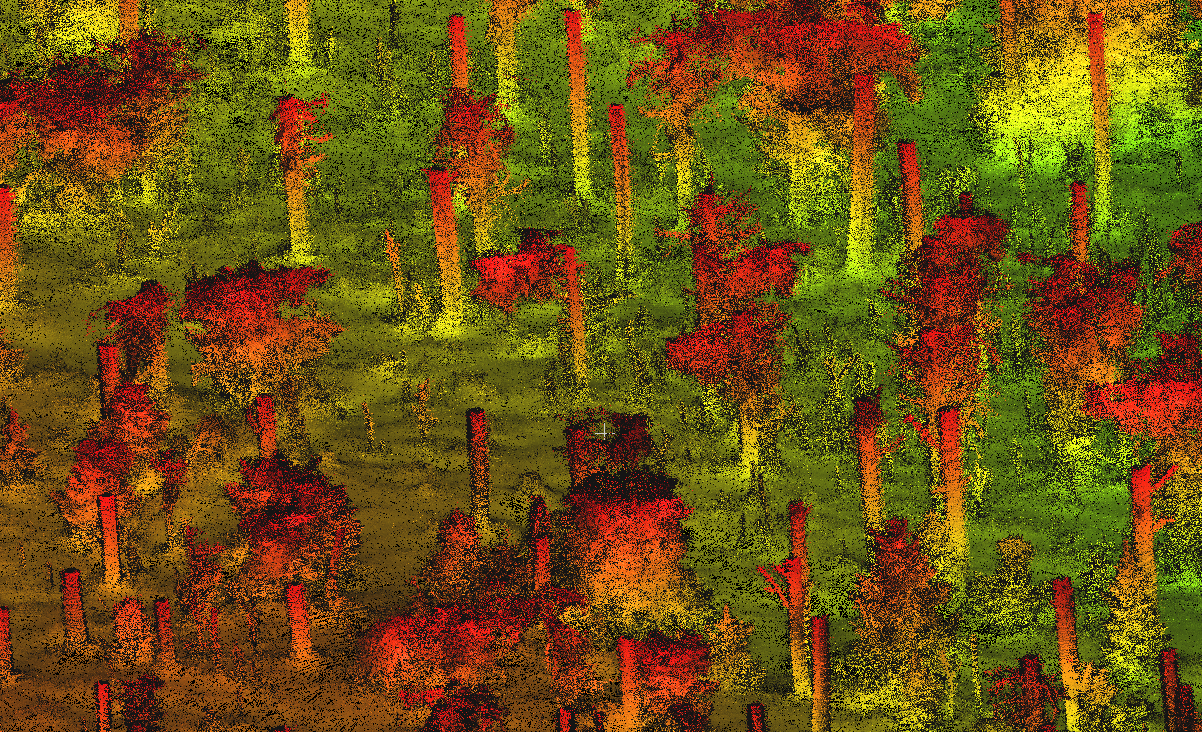
\includegraphics[width=0.49\columnwidth]{pics/exp_3_offline_pointclouds_trunk.png}
  % \caption{A region of Evo merged forest map point clouds coloured by height. I cropped canopies to check trunks of trees. Trunks are very distinct showing no evidence of drift occured.}
  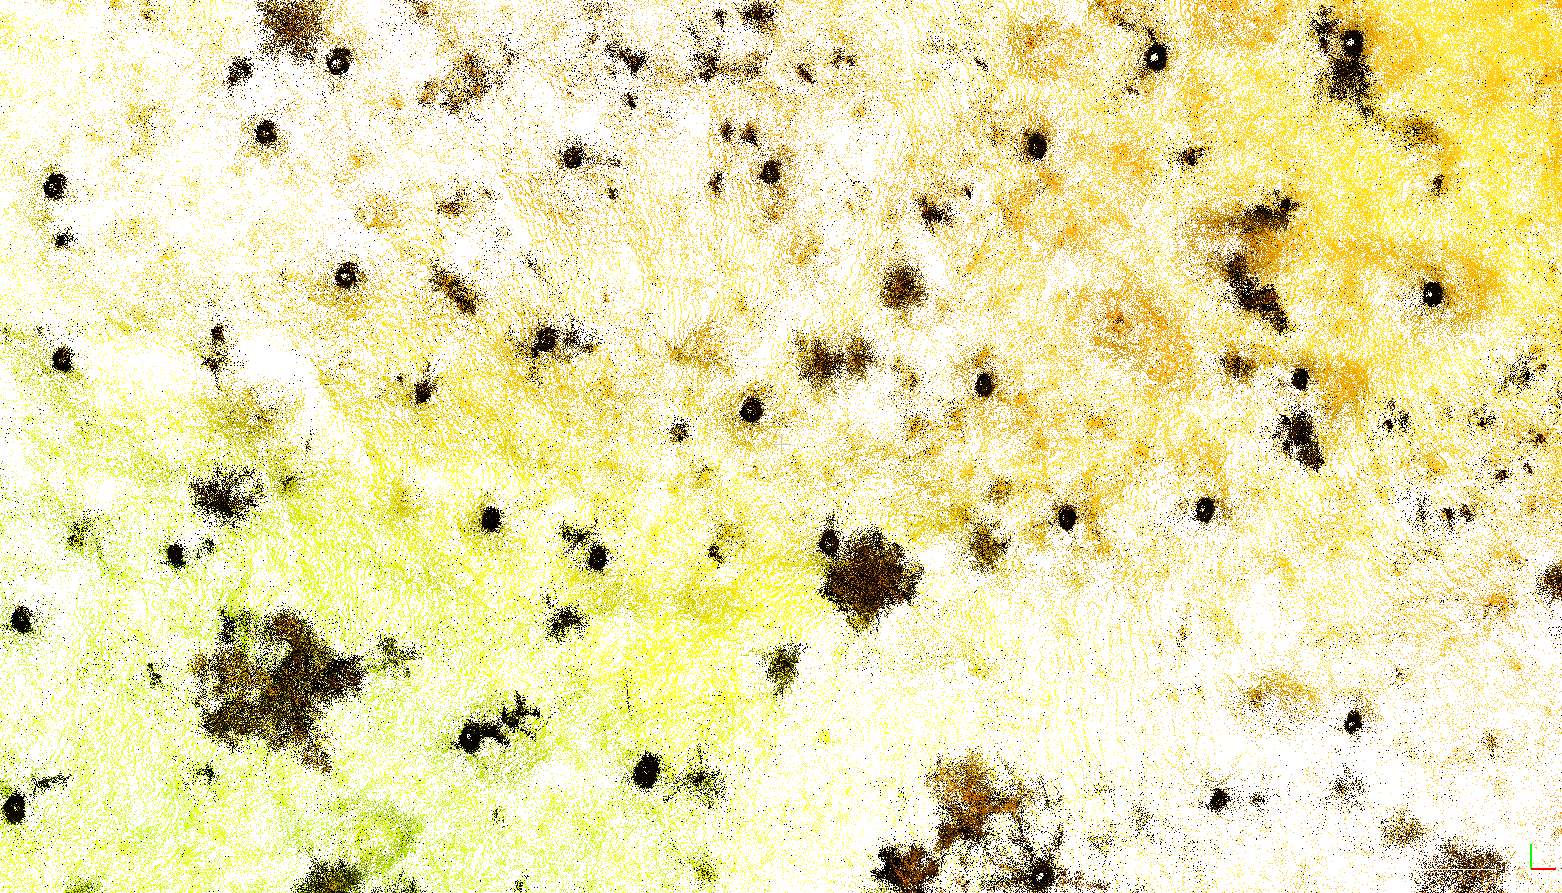
\includegraphics[width=0.49\columnwidth]{pics/exp_3_offline_pointclouds_trunk_BV3.png}
  \caption{Trunks of trees from Berd's eye view. We observed circular shapes for tree trunks clearly seen in the point clouds, indicating the map scanned in different viewpoints were registered correctly.}
  \label{fig:truk of trees}
\end{figure}
Overall, our experiments showed potential for efficient large-scale mapping, as we did not require to start at the open access roads nor following exactly the same paths to achieve loop closures between inter-missions. We also built the map incrementally, one section at a time, hence overlapping areas could only be guaranteed for subsequent missions.



% \tabref{tab:exp_offline_distance_table} provides summary statistics of the distribution of loop closures at different distance ranges. Our multi-stage verification pipeline effectively filters out unreliable loop candidates, with approximately 90\% of successful candidates found within 10\,m of each other. Notably, experiments conducted in Wytham Woods and the Forest of Dean highlight that our system can identify loop closures within the forests, eliminating the need to precisely retrace previously mapped areas to achieve loop closures. This underscores the versatility and robustness of our approach in real-world forest mapping scenarios.


% \begin{figure*}[htbp]
%   \centering
%   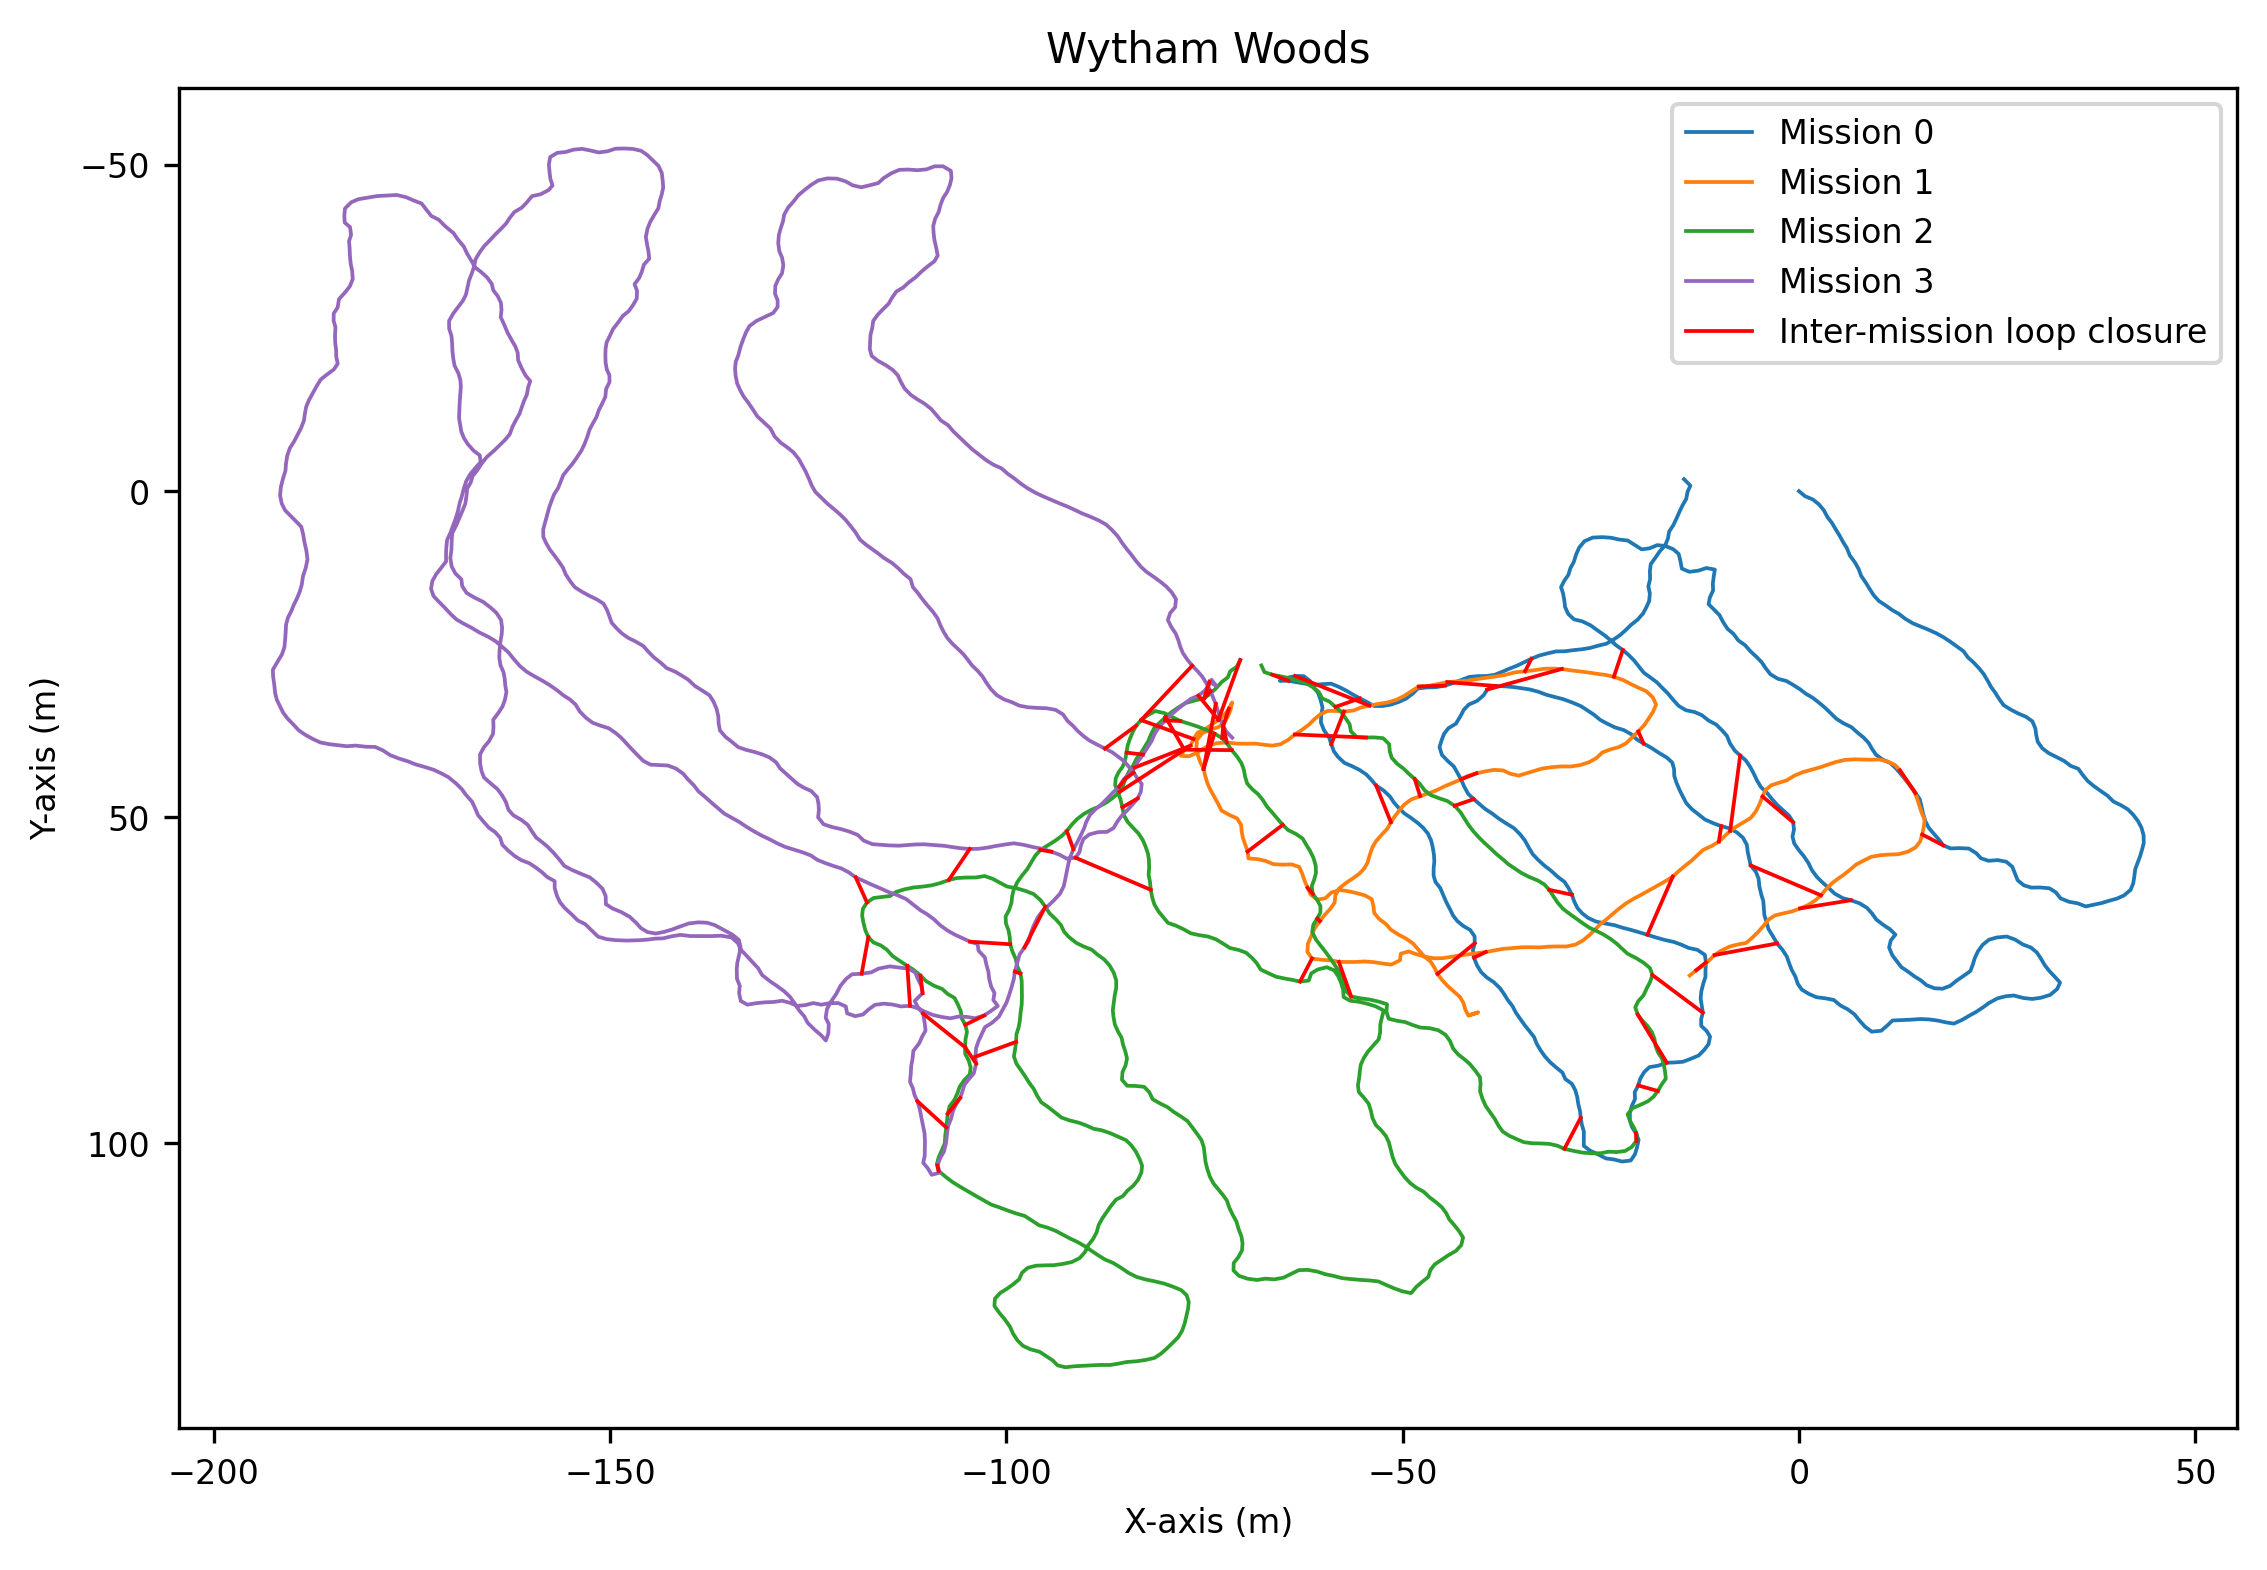
\includegraphics[width=0.90\columnwidth]{pics/exp_3_1_multimission_slam_wytham.png}
%   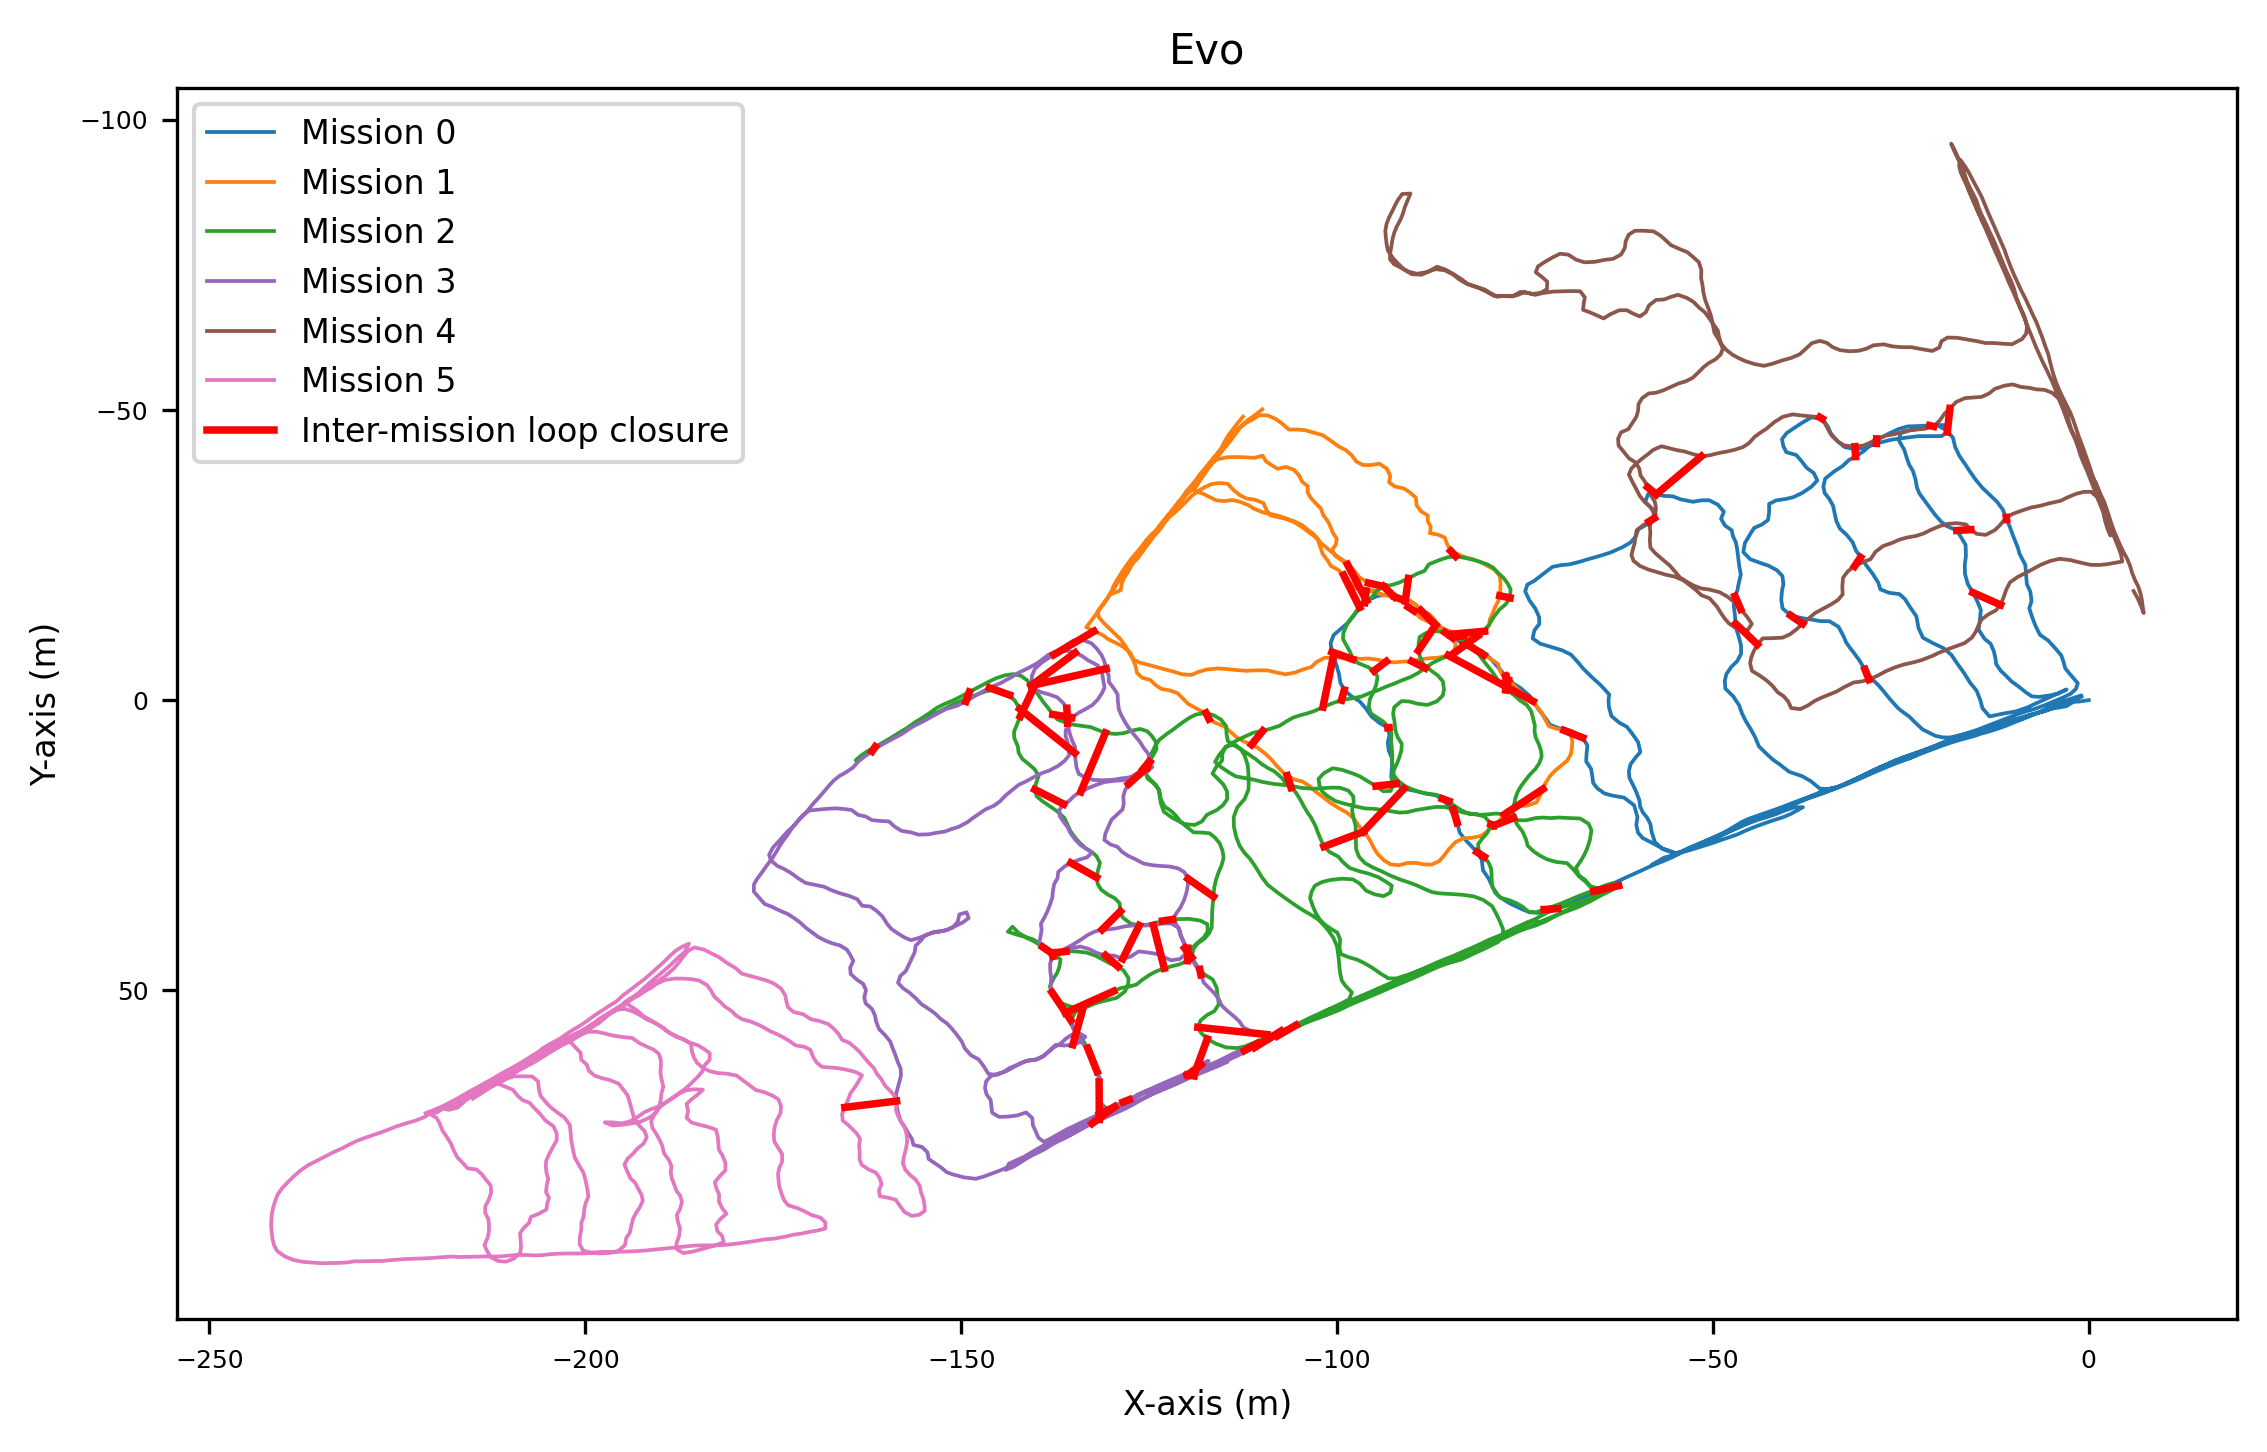
\includegraphics[width=0.90\columnwidth]{pics/exp_3_1_multimission_slam_evo.png}
%   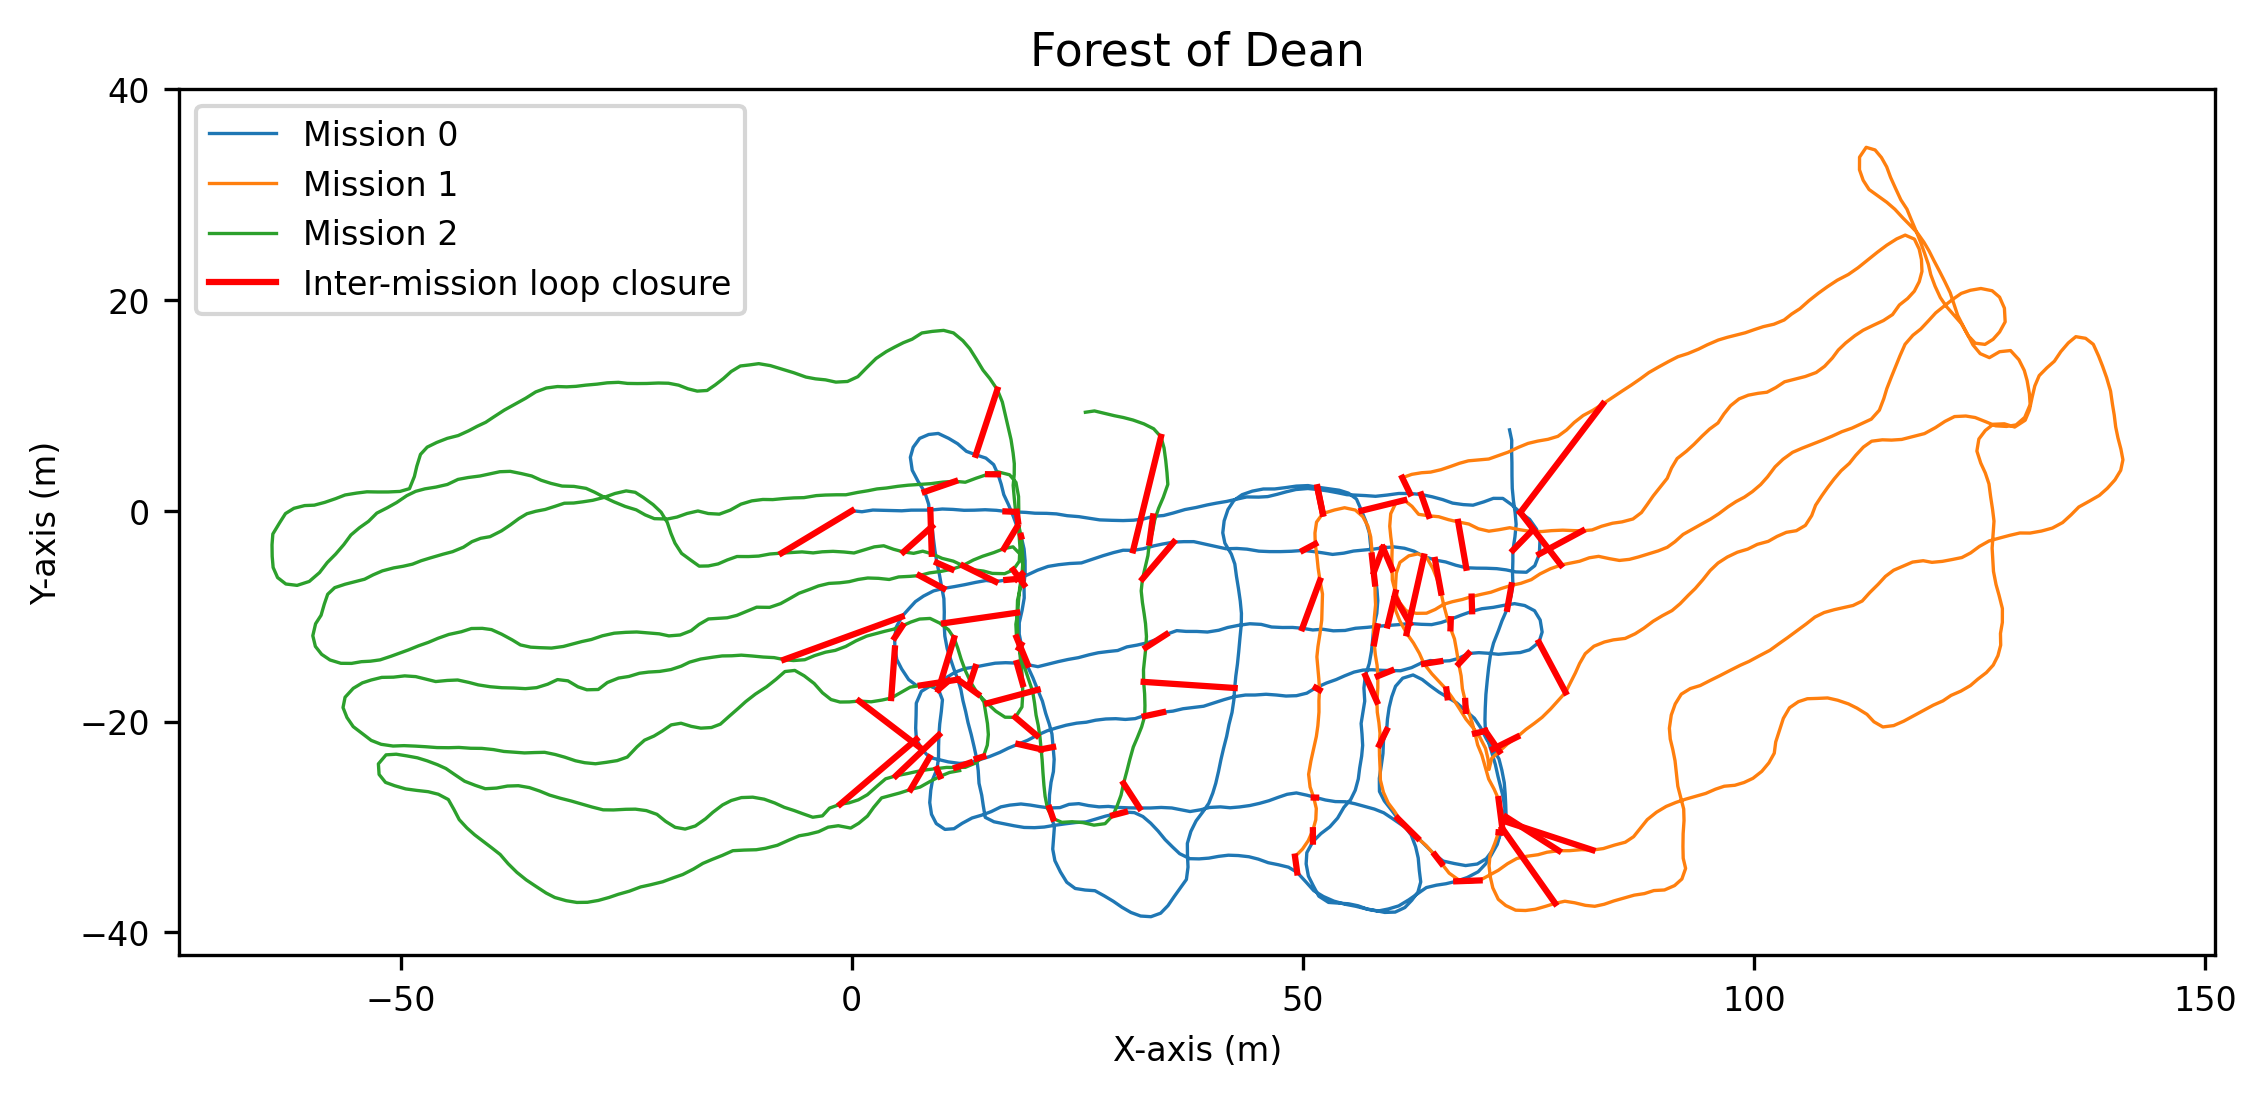
\includegraphics[width=0.90\columnwidth]{pics/exp_3_1_multimission_slam_dean.png}
%   \caption{Offline multi-mission SLAM. Left: Wytham - a densely wooded area with uneven terrain, including hills. Center: Evo - featuring a LiDAR setup on an incline, with loop closures occurring primarily when viewpoints are closely aligned. Right: Forest of Dean - flatter terrain compared to Wytham, with a sparser plantation, allowing for loop closures to be captured at greater distances. }
%   \label{fig:exp_multi_mission}
% \end{figure*}


% \begin{table}[htbp]
%   \centering
%   \small
%   \begin{tabular}{p{2cm}cccc}
%       \toprule
%       \multicolumn{1}{l}{loop closures} & \multicolumn{3}{c}{Dataset} \\
%       \multicolumn{1}{l}{distance range (m)} & Wytham & Evo & Forest of Dean \\
%       \midrule
%       0-5\,m &41 / 53\%  &83 / 78\%  &73 / 78\% \\
%       \midrule
%       5-10\,m &29 / 37\%  &19 / 18\% &15 / 16\%\\
%       \midrule
%       10-15\,m &8 / 10\%  &4 / 4\%   &6 / 6\% \\
%       \midrule
%       Total  & 78 / 100\%  & 106 / 100\%  & 94 / 100\% \\
%       \bottomrule
%   \end{tabular}
%   \caption{Offline Multi-mission map merging results corresponding to \figref{fig:exp_multi_mission}: Number and percentage of final inter-mission loop closures detected by distance between matched poses.}
%   %Setting rigorous thresholds on number of descriptors, SGV, pairwise consistency check and ICP registration allows robust loop-closure pairs to be found, with any loop-candidates more than 15m away rejected  
%   \label{tab:exp_offline_distance_table}
% \end{table}




% Fourth experiment: Relocalization 
\section{Relocalization} 
\label{sec:exp_relocalization}
% What is this experiment about?
This experiment showcases a relocalization demonstration in a dense forest using our approach. In this scenario, our system demonstrates the ability to continuously track the position within a prior SLAM map once an initial loop closure is established. Unlike multi-mission, since prior map poses are fixed as ground truth,  we no longer jointly optimize poses.
Instead, we try to relocalize the robot into the prior map using the current LiDAR scan and the prior map of individual scans. We set the pairwise consistency threshold at few centimeter level to enable consistent relocalization only within centimeter level of error. 
\begin{figure}[htbp]
  \centering
  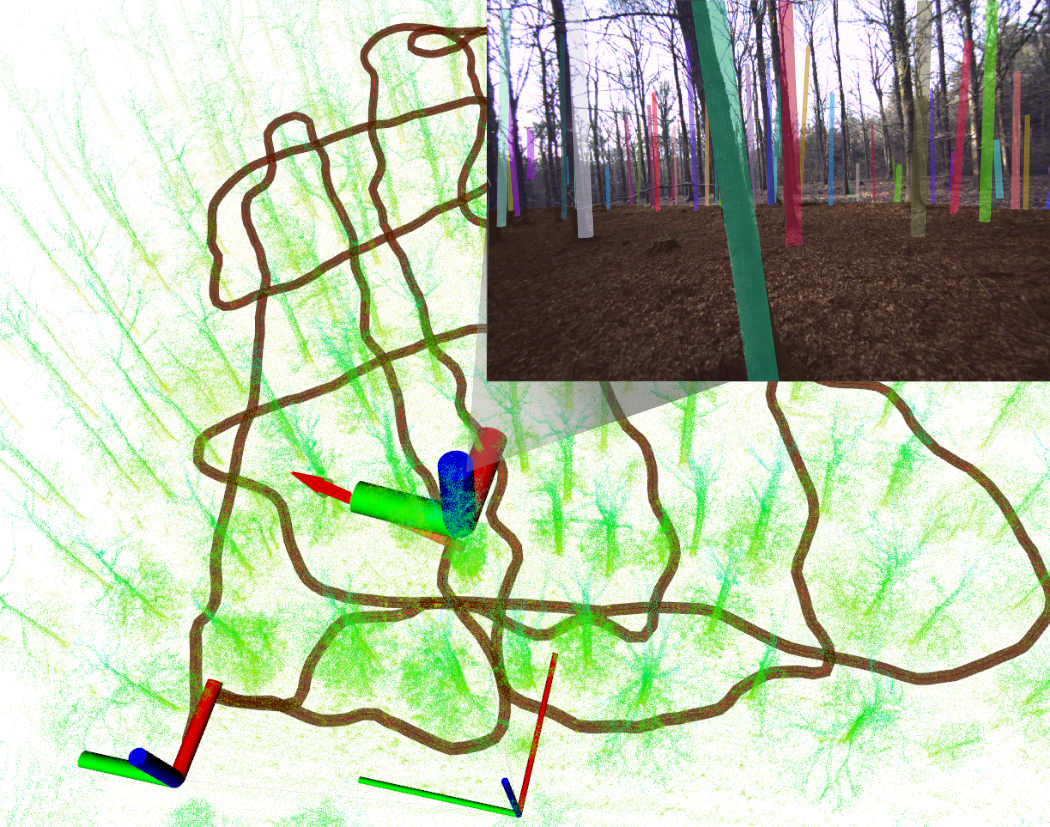
\includegraphics[width=0.80\linewidth]{pics/exp_4_relocalization_demo.png}
  \caption{Demonstration of relocalization capability. LiDAR (illustrated by large marker) is relocalized in a prior map (Dark Brown). We render a virtual view of the forest digital map synchronized with images from our camera (right). Red arrow shows a successful localization at that pose.}
  \label{fig:relocalization_demo}
\end{figure}

\subsection*{Forest Surveying Demonstration}
\figref{fig:relocalization_demo} and \figref{fig:relocalization_before_after} present illustrative examples of this demonstration, where the quadruped robot shown in \figref{fig:relocalization_before_after} is localized with respect to a prior SLAM map generated using a backpack LiDAR system. Drifts accumulated in the robot are corrected by finding loop candidates in the prior map of individual scans. This capability enables the real-time rendering of a virtual forest map overlaid with associated data, such as Diameter at Breast Height (DBH) and species information, onto the camera images. Such feedback is highly beneficial for tasks such as taking forest inventories by foresters or enabling autonomous harvesting.
\begin{figure}[htbp]
  \centering
  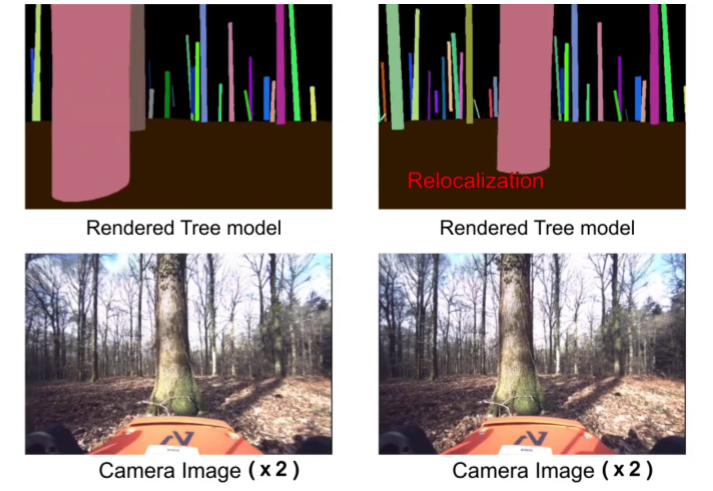
\includegraphics[width=0.99\linewidth]{pics/exp_4_relocalization_before_after.pdf}
  \caption{Demonstration of relocalization of a quadruped robot before and after.}
  \label{fig:relocalization_before_after}
\end{figure}

\subsection*{Relocalization Failure}
In relocalization scenario, relocalizing to incorrect candidate leads to a sudden jump in current base sensor position. This is easily detected by checking pairwise cycle consistency between map and base sensor. \figref{fig:relocalization_pairwise_cycle_consistency} shows an example of relocalization failure due to incorrect loop candidate (Left) and re-corrected by filtering out incorrect loop candidate (Right) checking pairwise cycle consistency.
\begin{figure}[htbp]
  \centering
  \includegraphics[width=0.99\linewidth]{pics/exp_4_relocalization_pairwise_before_after.pdf}
  \caption{Failure of relocalization due to incorrect loop candidate (Left). Correct relocalization after filtering out incorrect loop candidate by pairwise cycle consistency checking (Right).}
  \label{fig:relocalization_pairwise_cycle_consistency}
\end{figure}

% \subsection*{Time \& Distance to relocalize}
% We checked how long it takes to relocalize and how far the robot can move before relocalization fails.
%%%%%%%%%%%%%%%%%%%%%%%%

\section{Discussion \& Ablation Studies}

\subsection*{Study of ICP inlier-based check}
\label{sec:exp_icp_ablation}
Our final experiment investigates the ICP inlier-based check on loop closure integration within the final pose graph optimization process. This analysis is crucial for ensuring that incorrect loop closures are not introduced into the optimized pose graph.
\figref{fig:icp_inliers} illustrates the corrections (on top of the initial transformation prior) as estimated by the ICP registration at various distances. Additionally, the figure color-codes the points based on the number of inlier points obtained during the registration process, with blue indicating a large number of inliers and red indicating a smaller number.
Our observation suggests that loop closures occurring beyond 10\,m, which propose a substantial transformation correction often have fewer inlier ICP points and are thus less reliable.
Based on this analysis, we establish an inlier threshold to ensure that corrections are limited to ICP corrections of less than 1 meter (shown in dotted red line). This threshold further reduces the number of incorrect loop closures from being integrated into the pose graph.
\begin{figure}[t]
  \centering
  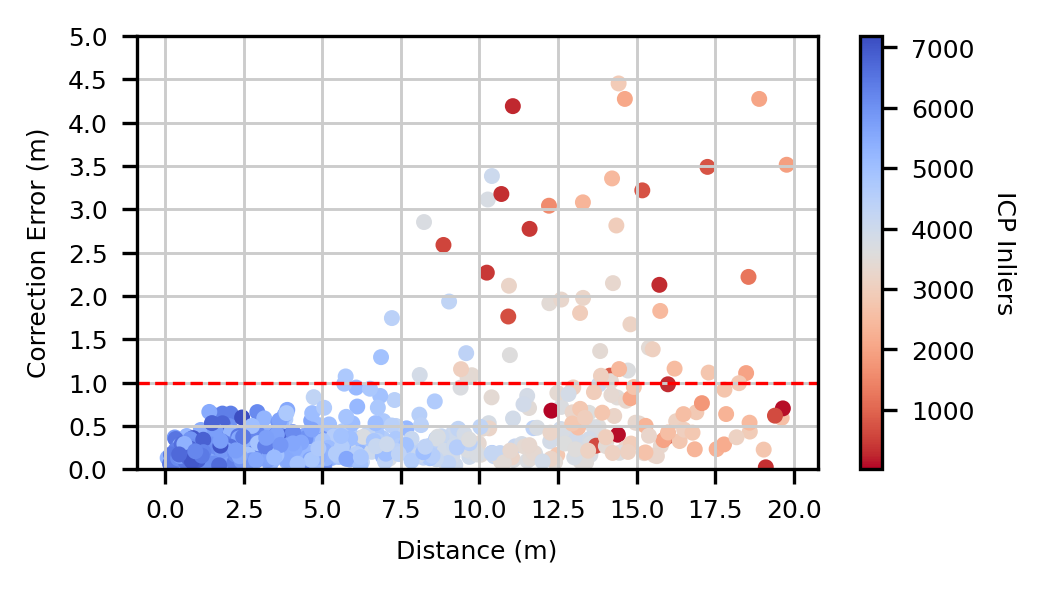
\includegraphics[width=0.99\linewidth]{pics/exp_4_ablation_icp_inliers_4cm}
  \caption{Analysis of final ICP registration check. X-axis shows the distribution of loop-candidates by distance after ICP.
  Y-axis shows ICP correction error w.r.t. the coarse-registration from RANSAC. Color indicates the number of ICP inliers,  30 iterations and RMSE= 0.01m, where clouds are cropped 50 by 50m, then downsampled to 20k points.}
  \label{fig:icp_inliers}
\end{figure}
 The ICP inliers threshold is fine tuned to $\sim$ 3k-5k points depending on the LiDAR setup and forest environments. There is trade-off between the baseline distance and the robustness of the loop-closure as shown in \figref{fig:icp_inliers_num}. For an example, in the Evo dataset, we set the threshold to 3k points, whereas in the Wytham Woods, we set the higher threshold to 4k-5k points. 
 \begin{figure}[t]
  \centering
  \includegraphics[width=0.99\linewidth]{pics/exp_4_icp_inliers_num1.pdf}
  \caption{Loop closure distribution by distance at various ICP inlier thresholds. Blue lines are accepted loop candidates and Red lines are rejected candidates. Stricter(higher) ICP inlier threshold will provide more robust loop-closures but baseline distance will be shorter, whereas lower ICP inlier threshold will provide far distance loop-closures but there is a chance of getting False Positives.}
  \label{fig:icp_inliers_num}
\end{figure}
% What is the interpretation of the figure?
% Alongside \figref{fig:exp_2_2_loop_closure_histograms}, further analysis has been done how robust the loop-candidates are. 
% \figref{fig:ablation_icp_inliers} shows that under 10m distance, ICP inliers are high as over 4k points, and correction error is below 1m. However, the distribution of loop-candidates start to diverge significantly after 10m: correction error no longer bounds to 1m and the number of inliers are much less than 4k points. 
% Setting a low ICP inlier threshold will provide far distance loop-closures, but there is a chance of getting False Positives.
\subsection*{Computation Analysis}
\textbf{Runtime Analysis}\hspace{0.5em} Currently the system requires a GPU for descriptor extraction. The system runs at 0.73 Hz on a laptop with an Intel i7-10750H CPU and an NVIDIA RTX A3000 GPU. The processing time for the top-1 loop closure candidate detection is shown in \tabref{tab:my-table}. The descriptor extraction and RANSAC featuring matching are the most time-consuming process, thus running below 1Hz. It is not ideal for real-time applications, but it is sufficient for offline processing. 
\begin{table}[h]
  \centering
  \small
  \begin{tabular}{@{}llllll@{}}
  \toprule
  \textbf{Process} & \textbf{Prep.} & \textbf{Desc.} & \textbf{SGV} & \textbf{Reg.} & \textbf{Total} \\ \midrule
  \textbf{Avg. Time (s)} & 0.015 & 0.09 & 0.001 & 1.1 & 1.3 / 0.73 Hz \\
  \bottomrule
  \end{tabular}
  \caption{Avg. processing times for various tasks. (Prep.-Preprocessing, Desc.-Descriptor Extraction, Reg.-RANSAC Registration.)}
  \label{tab:my-table}
\end{table}
\newline
\textbf{Memory Consumption}\hspace{0.5em} Dimension of global and local descriptor is 1028 and (N,256) respectively (N is the number of keypoints). This means one global descriptor requires only 8 bytes of memory, and one local descriptor requires $\sim$2KB of memory. The memory consumption of the system is mainly dominated by the local descriptors, which are stored in the GPU memory. One seuqnece of run ($\sim$1000 scans) requires $\sim$2GB of GPU memory.

\subsection*{Hyper Parameters}
\textbf{Voxel Size}\hspace{0.5em} During preprocessing step it is necessary to voxelize input point clouds for discritize representation using \emph{MinkowskiEngine~\cite{choy20194cvpr}, SparseTorch~\cite{tang2023MICRO} with CUDA}. This voxel size is known to be critical for the performance of the model descriptors. Since both Logg3dNet and EgoNN are trained on WildPlace dataset, which is different from our dataset in terms of density and range of LiDAR point clouds, We empirically determined the optimal voxel size between \SIrange{0.1}{1.0}{\meter} through direct experimentation on our dataset. Tab.~\ref{tab:voxel_size} shows that optimal voxel sizes are \SI{0.1}{\meter} and \SI{0.6}{\meter} for Logg3dNet on Evo dataset. Since the difference is not significant, we decided to use voxel size of \SI{0.6}{\meter} considering computational efficiency.\\

\begin{table}[htbp]
  \centering
  \begin{tabular}{p{2cm} *{6}{c}}
      \toprule
      \multicolumn{1}{l}{Testing} & \multicolumn{6}{c}{Voxel size (cm)} \\
      \cmidrule{2-7}
      \multicolumn{1}{l}{Datasets} & 10 & 20 & 40 & 60 & 80 & 100 \\
      \midrule
      Evo-12 &\textbf{0.89} &0.79 &0.77 &\textbf{0.86} &0.79 &0.78 \\
      \addlinespace % Add space between rows
      Evo-16 & \textbf{0.74} & 0.66 & 0.66 & \textbf{0.66} & 0.64 & 0.63 \\
      \addlinespace % Add space between rows
      Evo-18  &0.71 & 0.75 & \textbf{0.75} & \textbf{0.76} & 0.73 & 0.71 \\
      \bottomrule
  \end{tabular}

  \caption{$F{1}_{max}$ score of Logg3dNet with different voxel sizes on Evo dataset. Bold numbers indicate the best and second best $F{1}_{max}$ score.}
  \label{tab:voxel_size}
\end{table}

  
\textbf{LI-OSAM Odometry System}\hspace{0.5em} We plan to test \emph{Place Recognition Server} with other LiDAR-intertial odometry systems such as LIOSAM~\cite{shan2020iros} to evaluate the robustness of the system in different environments. LIOSAM is a LiDAR-intertial odometry system that can provide accurate odometry information in various environments, including dense forests. We will evaluate the performance of the system with LIOSAM in the future.

